%--------------------------------------------------------------------------------
%--------------------------------------------------------------------------------
%    CHAPTER II: THEORY OF COMPUTATION
%--------------------------------------------------------------------------------
%--------------------------------------------------------------------------------

\part*{Theory of Computation}
\addcontentsline{toc}{part}{\tocpartglyph Theory of Computation}

\vspace{\baselineskip}
\begin{displayquote}
	\textit{Theory is relevant to you because it shows you a new, simpler, and more elegant side of computers, which we normally consider to be complicated machines. The best computer designs and applications are conceived with elegance in mind. A theoretical course can heighten your aesthetic sense and help you build more beautiful systems.}
	\begin{flushright}
		---Michael Sipser
	\end{flushright}
\end{displayquote}
\vspace{4mm}

% Mathematical modeling of computation (sequential, functional, concurrent)
% Automata theory covers sequential and concurrent, computability theory covers functional. Together, they cover the prominent models of computations.
% Computational complexity theory is a categorization of computational tasks.

The \textit{theory of computation} is a field of study that is related to both mathematics and computer science. It is concerned with a process known as \textit{computation}, which refers to any kind of \textit{calculation} (the transformation of one or more inputs into one or more outputs) that is accomplished by following an \textit{algorithm} (a set of rigorously defined steps). It is also concerned with the formalization of theoretical models of computation known as \textit{abstract machines} or \textit{abstract automata}. Also of interest are the \textit{computational problems} that can be solved by these abstract machines and how efficiently they can be solved. The theory of computation gives us the formal definition of a computer and the scope of what a computer can accomplish. \\

Much of the work in the theory of computation is$\dots$ quite abstract. While calculation and computation have been practiced by humans for thousands of years, the concept was only formalized by mathematicians, logicians, philosophers, linguists, and computer scientists in the past 150 years. This part of the guide will delve into some fairly academic topics with a decent amount of mathematical rigor, but it is written to be accessible and entertaining. \\

The field has three branches: \textit{automata theory}, \textit{computability theory}, and \textit{computational complexity theory}, each of which asks fundamental questions pertaining to how mathematical calculations can be automated, which kinds of problems can be solved by a machine, and how many resources are required to solve a particular problem. We will touch on the major discoveries made in each of these branches and discuss why they are significant to computer science and programming in general.

% "Graduate-level mathematics"

%--------------------------------------------------------------------------------
%    SECTION: AUTOMATA THEORY
%--------------------------------------------------------------------------------

\toclineskip
\section{Automata Theory}

% Concept of automata
% Models of computation
% Computation requires state, transition, and language

\textit{Automata theory} is the study of \textit{automata} and their behavior. An \textit{automaton} is a self-operating machine designed to follow or respond to a predetermined sequence of operations. Automata include physical devices such as cuckoo clocks, mechanical watches, robots, and computer processors as well as \textit{abstract machines}. An abstract machine is any formal description of \textit{mechanical behavior}. An abstract machine that is used to formally describe computation is called a \textit{model of computation}. This is a mathematical description of what a computer is, and it models the computation that a real, concrete computer could actually perform, if you were to implement that computer according to the model's specifications. Like their concrete counterparts, abstract machines have \textit{state}, a set of information in the \textit{present} that was acquired due to \textit{past} events. All automata begin with a \textit{starting state}, receive some sort of \textit{input}, and \textit{transition} to another state based on the value of that input and the value of its current state. \\

One \textit{abstract automaton} in particular fully models not only the computation that is performed by today's state-of-the-art computers, but also the very process of computation itself. We will spend a lot of time in this guide discussing the structure and behavior of this model as well as what its limitations imply regarding the future of computing, software, mathematics, and the meaning of life. We will also briefly explore the abstract automata that exist in pure mathematics and model computation that is not physically realizable. \\

%----------------------------------------

\subsection{From Knots to Nodes}

% Explain what graphs are so you can use them to model automata.

It is worth pausing here to think about what the word \textit{node} really means. It comes from the Latin word \textit{nodus}, which means \textit{knot}. A node is like a knot in a string: a distinguishable lump at a certain position. And between any two adjacent knots in a string, there is a \textit{link} \dots\ of string. Similarly, between any two adjacent links, there is a knot. \\

The knots and the links cannot exist independent of each other. Without knots, there are no links of string---just one, continuous string. Without links, knots are totally unanchored and have no sense of position. Now, one could argue that a single knot is sufficient for the existence of links in a string, but such a view is naive and presumes a familiar, everyday sort of string. \\

For example, yes, you can tie a single knot in a shoelace, and you might then call the floppy bits on either side of it "links." But when you call something like this a link, what you are really pointing out is its \textit{finite length}. That is, the "string link" \textit{starts} at the knot and \textit{ends} at the tip of the aglet. But length is a nonessential detail for links---the essence of a \textit{link} is its \textit{connecting} of things. A better term in this case would be \textit{loose end} or simply \textit{end}. A knot with two loose ends is shown below: \\

\begin{center}	
	\begin{tikzpicture}[scale=0.2]
	\begin{knot}[
	consider self intersections,
	flip crossing=2
	clip width=5,
	]
	\strand[ultra thick]
	(90:1.25) to[out=180,in=-120,looseness=2]
	(-30:1.25) to[out=60,in=120,looseness=2]
	(210:1.25) to[out=-60,in=0,looseness=2] (90:1.25);
	\end{knot}
	
	\draw [ultra thick, dashed] (-1.2,0) -- ++(-5,0);
	\draw [ultra thick, dashed] (1.2,0) -- ++(5,0);
	\end{tikzpicture}
\end{center}

For our purposes, it is better to envision a taut string that stretches to infinity in both directions and to think of a \textit{link} as a \textit{connector of a knot pair} whose length may or may not be important. With this model, there must be at least two knots in the string if we are to think of them as \textit{nodes} (i.e. things that are connected to something else). A string with five \textit{trefoil} (three-leafed) knots and four links is shown below: \\

\begin{center}
	\begin{tikzpicture}[scale=0.2]
	\foreach \x in {-2,-1,0,1,2} {
		\begin{knot}[
		consider self intersections,
		flip crossing=2
		clip width=5,
		xshift=\x*250,
		]
		\strand[ultra thick]
		(90:1.25) to[out=180,in=-120,looseness=2]
		(-30:1.25) to[out=60,in=120,looseness=2]
		(210:1.25) to[out=-60,in=0,looseness=2] (90:1.25);
		\end{knot}
	}
	
	\foreach \x in {-1,0,1,2} {
		\draw [ultra thick] (-1.2+\x*8.75,0) -- ++(-6.45,0);
	}
	\draw [ultra thick, dashed] (-18.75,0) -- ++(-9,0);
	\draw [ultra thick, dashed] (18.75,0) -- ++(9,0);
	\end{tikzpicture}
\end{center}

In the mathematical field of \textit{knot theory}, knots are defined similarly, but they do not have ends. That is, a mathematical knot is defined as a \textit{closed} circle embedded in a three-dimensional Euclidean space and subject to continuous deformation. Essentially, this means that you can cut a circular string at a point, tangle it, and close the circle at the same point to form any mathematical knot you like. The process of tying a \textit{cinquefoil}, a knot with five \textit{crossings}, is given below as an example: \\[\baselineskip]

\resizebox{\textwidth}{!}{
	\begin{tikzpicture}
	\draw[very thick] (0,0) circle (2);
	\filldraw[line width=1mm,textbook-blue] (0,0) ++(60:2) arc (60:70:2);
	
	\begin{knot}[
	consider self intersections,
	flip crossing=2
	clip width=5,
	xshift=150
	]
	\strand[very thick] (2,0) .. controls +(0,1.0) and +(54:1.0) .. (144:2) .. controls +(54:-1.0) and +(18:-1.0) .. (-72:2) .. controls +(18:1.0) and +(162:-1.0) .. (72:2);
	\end{knot}
	
	\begin{knot}[
	consider self intersections=true,
	%  draft mode=crossings,
	flip crossing/.list={2,4},
	only when rendering/.style={
		%    show curve controls
	},
	xshift=300
	]
	\strand[very thick] (2,0) .. controls +(0,1.0) and +(54:1.0) .. (144:2) .. controls +(54:-1.0) and +(18:-1.0) .. (-72:2) .. controls +(18:1.0) and +(162:-1.0) .. (72:2) .. controls +(162:1.0) and +(126:1.0) .. (-144:2);
	\end{knot}
	
	\begin{knot}[
	consider self intersections=true,
	%  draft mode=crossings,
	flip crossing/.list={2,4},
	only when rendering/.style={
		%    show curve controls
	},
	xshift=450
	]
	\strand[very thick] (2,0) .. controls +(0,1.0) and +(54:1.0) .. (144:2) .. controls +(54:-1.0) and +(18:-1.0) .. (-72:2) .. controls +(18:1.0) and +(162:-1.0) .. (72:2) .. controls +(162:1.0) and +(126:1.0) .. (-144:2) .. controls +(126:-1.0) and +(0,-1.0) .. (2,0);
	\end{knot}
	\end{tikzpicture}
} \\[\baselineskip]

% There are no ends for each knot. A single knot is closed. Links are not like above.

Note that because mathematical knots are closed, they cannot be linked together like knots in a string. Instead, a link in knot theory is a collection of knots that are knotted together. \\

% We, however, are interested in the more general \textit{graph theory}, whose focus is on how knots are connected to other knots rather than on the structures of the knots themselves. A \textit{graph} is a drawing of objects and relations in which each object or \textit{node} is represented by a circle and each relation or \textit{link} is represented by a line or arrow. \\

% The string above can be thought of as a list. Here are some other structures that are graphs (tree, grid, two linked knots)

% Node is a joint or a communication hub in an information system. It is connected to other nodes by links or communication channels. Node is Latin for knot. So node/connection in information science, vertex/edge in graph theory.

% Calculation vs computation. Separate histories.
% Is a microwave a computer?
% Modern cars are full of computers. Embedded systems.

%----------------------------------------

\subsection{Exploring the Link Between Concrete and Abstract Machines}

Let's take a simple, concrete machine and try to visualize the abstract machine that underlies it. Consider a cuckoo clock. Every day, at noon, a small plank with a mechanical bird perched on its lip will extend from a hole above the clock face, powered by a working motor. Once the plank is fully extended, the bird will flap its metal wings and maybe turn its head as a song is played from a revolving music box inside the clock. Then, when it is 12:01 PM, the music will stop, the bird will still, and the plank will retract. The process will occur again the next day, at noon. \\

The machine's components here are the plank, the bird, and the music box. The components each have two states: the plank can be retracted or extended, the bird can be still or flapping its wings, and the music box can be paused or playing. The input to this machine is whether or not the clock hands both point straight at 12. We can say that this automaton has a state that can be expressed in terms of the states of its components. We can represent its starting state with the sequence (0,0,0) (i.e. the plank is retracted, the bird is still, and the music box is paused). The automaton can receive one of two inputs, 1 or 0 (i.e. both clock hands point straight at 12 or they do not). This input might be implemented with an electromechanical switch that turns the motor on or off.

\paragraph{(0,0,0) -> (1,0,0)} We start at state (0,0,0). As the morning passes, the automaton receives a constant input of 0, which keeps it in its starting state. At noon, the input switches to 1, and the automaton transitions to the state (1,0,0). As the plank extends and transitions its own state from 0 to 1, the bird remains still, and the music box remains paused. Once the plank is fully extended, we are in state (1,0,0).

\paragraph{(1,0,0) -> (1,1,1)} We expect that the plank will be fully extended well before 12:01 PM, so the input should still be 1. However, if for some reason the input is 0, we should transition back to (0,0,0), as the machine should only operate outside of its starting state between 12:00 and 12:01 PM. This is a simple example of \textit{strange input}. The input 0 at this state is unexpected, but it is technically possible. It is a better idea to define the behavior for this unexpected case, rather than to allow the input to cause unexpected behavior. On the other hand, if the input is 1 at this state, the automaton transitions to the state (1,1,1). The plank is fully extended, the bird is flapping its wings, and the music box is playing.

\paragraph{(1,1,1) -> (0,0,0)} Before 12:01 PM, the input is still 1, and that input should keep the automaton in its current state of (1,1,1). When 12:01 PM rolls around, the input will now be 0. In this case, we would like to return to the original state. On receipt of the input 0 while in state (1,1,1), the automaton transitions back to its starting state, (0,0,0). This abstract machine is shown below with a state format of (plank, bird, music) and an input specifying if the clock hands point exactly toward 12.

% Drawing of "Bad Automaton"
\begin{center}
	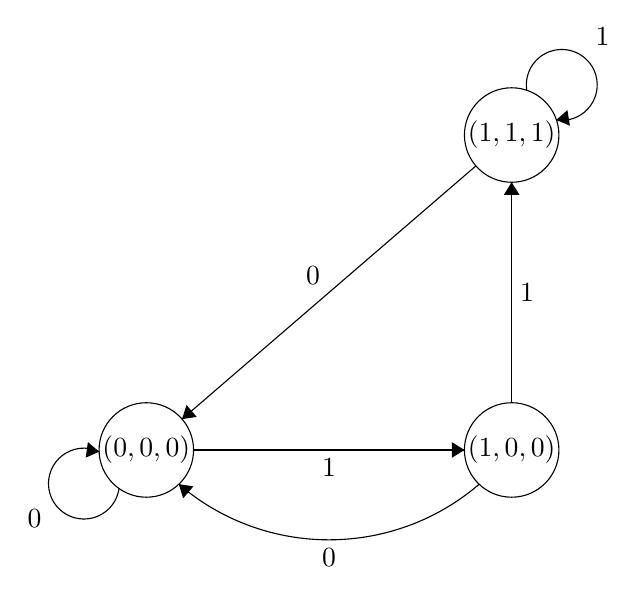
\begin{tikzpicture}[scale=0.2]
	\tikzstyle{every node}+=[inner sep=0pt]
	\draw [black] (28.4,-36.5) circle (3);
	\draw (28.4,-36.5) node {$(0,0,0)$};
	\draw [black] (51.6,-36.5) circle (3);
	\draw (51.6,-36.5) node {$(1,0,0)$};
	\draw [black] (51.6,-16.5) circle (3);
	\draw (51.6,-16.5) node {$(1,1,1)$};
	\draw [black] (31.4,-36.5) -- (48.6,-36.5);
	\fill [black] (48.6,-36.5) -- (47.8,-36) -- (47.8,-37);
	\draw (40,-37) node [below] {$1$};
	\draw [black] (51.6,-33.5) -- (51.6,-19.5);
	\fill [black] (51.6,-19.5) -- (51.1,-20.3) -- (52.1,-20.3);
	\draw (52.1,-26.5) node [right] {$1$};
	\draw [black] (26.668,-38.935) arc (-7.69924:-295.69924:2.25);
	\draw (21.78,-40.87) node [left] {$0$};
	\fill [black] (25.41,-36.61) -- (24.69,-36) -- (24.55,-36.99);
	\draw [black] (49.539,-38.673) arc (-49.35642:-130.64358:14.645);
	\fill [black] (30.46,-38.67) -- (30.74,-39.57) -- (31.39,-38.81);
	\draw (40,-42.71) node [below] {$0$};
	\draw [black] (52.56,-13.67) arc (189:-99:2.25);
	\draw (56.9,-10.25) node [right] {$1$};
	\fill [black] (54.43,-15.54) -- (55.3,-15.91) -- (55.14,-14.92);
	\draw [black] (49.33,-18.46) -- (30.67,-34.54);
	\fill [black] (30.67,-34.54) -- (31.6,-34.4) -- (30.95,-33.64);
	\draw (38.99,-26.01) node [above] {$0$};
	\end{tikzpicture}
\end{center}
\vspace{5mm}

This is a perfectly reasonable abstract machine, but something isn't right. It does not accurately simulate the behavior of the cuckoo clock we described. What happens when the clock strikes midnight? The clock hands will point at 12, producing an input of 1, but we don't want the bird to wake everyone up at midnight. We could use two bits of input: whether or not the hands are between 12:00 and 12:01, and whether it is AM or PM. Additionally, the music never plays unless the bird is flapping its wings, so we can combine those states. The abstract machine is better represented by the diagram below with a state format of (plank, bird/music) and an input format of (hands are toward 12, is PM).

% Drawing of "Good Automaton"
\begin{center}
	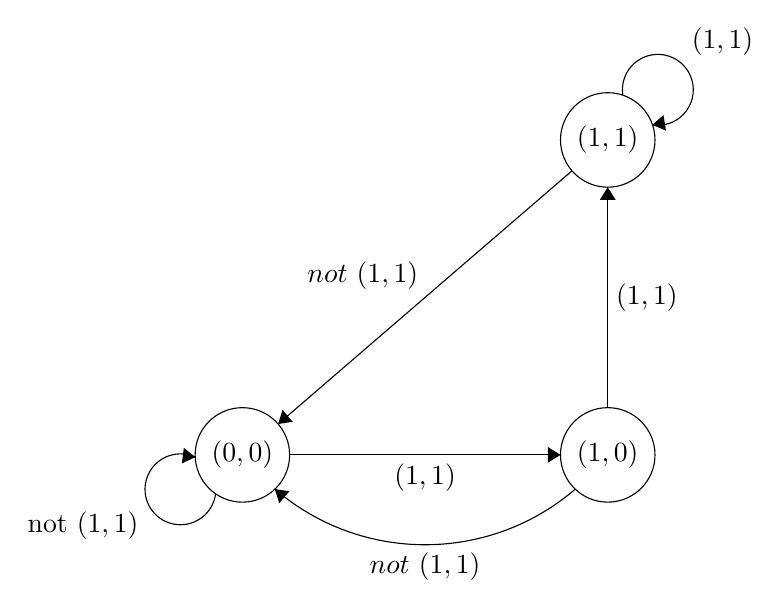
\begin{tikzpicture}[scale=0.2]
	\tikzstyle{every node}+=[inner sep=0pt]
	\draw [black] (28.4,-36.5) circle (3);
	\draw (28.4,-36.5) node {$(0,0)$};
	\draw [black] (51.6,-36.5) circle (3);
	\draw (51.6,-36.5) node {$(1,0)$};
	\draw [black] (51.6,-16.5) circle (3);
	\draw (51.6,-16.5) node {$(1,1)$};
	\draw [black] (31.4,-36.5) -- (48.6,-36.5);
	\fill [black] (48.6,-36.5) -- (47.8,-36) -- (47.8,-37);
	\draw (40,-37) node [below] {$(1,1)$};
	\draw [black] (51.6,-33.5) -- (51.6,-19.5);
	\fill [black] (51.6,-19.5) -- (51.1,-20.3) -- (52.1,-20.3);
	\draw (52.1,-26.5) node [right] {$(1,1)$};
	\draw [black] (26.699,-38.957) arc (-6.96472:-294.96472:2.25);
	\draw (21.83,-40.98) node [left] {not $(1,1)$};
	\fill [black] (25.42,-36.64) -- (24.68,-36.05) -- (24.56,-37.04);
	\draw [black] (49.539,-38.673) arc (-49.35642:-130.64358:14.645);
	\fill [black] (30.46,-38.67) -- (30.74,-39.57) -- (31.39,-38.81);
	\draw (40,-42.71) node [below] {$not\mbox{ }(1,1)$};
	\draw [black] (52.56,-13.67) arc (189:-99:2.25);
	\draw (56.9,-10.25) node [right] {$(1,1)$};
	\fill [black] (54.43,-15.54) -- (55.3,-15.91) -- (55.14,-14.92);
	\draw [black] (49.33,-18.46) -- (30.67,-34.54);
	\fill [black] (30.67,-34.54) -- (31.6,-34.4) -- (30.95,-33.64);
	\draw (36.05,-26.01) node [above] {$not\mbox{ }(1,1)$};
	\end{tikzpicture}
\end{center}
\vspace{5mm}

% Generalize this diagram to labelled transition system
% Transition system is a directed graph

% Transition system, semiautomaton, operator monoid
% F-coalgebra => transition systems are classes (math object)
% Difference between semiautomata and automata

Note that the actual complexity of the concrete cuckoo clock would be a bit more complicated than the automaton above. For example, what does the bird do specifically when it is on? Perhaps it raises and lowers its wings three times, turns its head to the right twice, and repeats. This process can be modeled by a different automaton. To fully model a concrete automaton, we must reduce it to an abstract machine, a system of states and transitions that account for every intended behavior. Abstract machines are capable of modeling systems of any arbitrary complexity. The automaton above is a model of computation called a \textit{finite-state machine} (FSM), and it will be the first abstract machine that we will discuss.
\\

% The nodes could themselves be automata => automata are recursive structures

%----------------------------------------

\subsection{Formalization of an Abstract Machine}

\begin{tcolorbox}[breakable, enhanced, colback=textbook-blue, sharp corners]
	\vspace{3mm}
	\begin{center}
		\textbf{A Brief Introduction to Formal Grammars}
	\end{center}
	A formal grammar is a finite set of \textit{production rules} that specifies what a particular language is supposed to look like. It formalizes the structure of "grammatical units" in a language. This is done in order to enforce a specific alphabet, a consistent lexicon, and a predictable sentence structure, all of which contribute to how useful and distinct any given language is. \\
	
	A grammar $G$ consists of the following components:
	\begin{itemize}
		\item A finite set $N$ of \textit{nonterminal} symbols.
		\item A finite set $\Sigma$ of \textit{terminal} symbols that is disjoint from $N$.
		\item A symbol $S\in N$, designated as the \textit{start symbol}.
		\item A finite set $P$ of \textit{production rules} where each rule is of the form ${(\Sigma\cup N)^*N(\Sigma\cup N)^*\rightarrow(\Sigma\cup N)^*}$.
	\end{itemize}
	
	Put another way, a production rule converts a sequence of symbols to another sequence of symbols. If a rule is of the form \textit{left-hand side $\rightarrow$ right-hand side}, each side can contain terminals and nonterminals, but its left-hand side must contain at least one nonterminal. A nonterminal is a symbol that is replaced by other symbols when an appropriate rule is applied. Unlike a terminal, it does not belong to the alphabet of the language, but rather represents a sequence of symbols that do. Terminals cannot be replaced by other symbols once chosen. \\
	
	Let's construct a simple formal grammar. It is typical for the nonterminals to be uppercase and for the terminals to be lowercase. Let $N=$ \{SENTENCE, NOUN, ADJ\}, $\Sigma=$ \{the, dog, building, plays, fluffy, good\}, and $S=$ SENTENCE. The rules of $P$ are given below.
	
	\begin{itemize}
		\item SENTENCE $\rightarrow$ the NOUN plays
		\item NOUN $\rightarrow$ ADJ NOUN
		\item NOUN $\rightarrow$ dog
		\item NOUN $\rightarrow$ building
		\item ADJ $\rightarrow$ fluffy
		\item ADJ $\rightarrow$ good
	\end{itemize}
	
	We can now start with SENTENCE and apply these rules to construct a "sentence" that is valid in this language. Example sentences and their derivations are given below.
	
	\begin{itemize}
		\item SENTENCE $\rightarrow$ the NOUN plays $\rightarrow$ the ADJ NOUN plays $\rightarrow$ the good NOUN plays $\rightarrow$ the good dog plays
		\item SENTENCE $\rightarrow$ the NOUN plays $\rightarrow$ the ADJ NOUN plays $\rightarrow$ the ADJ ADJ NOUN plays $\rightarrow$ the ADJ ADJ ADJ NOUN plays $\rightarrow$ the fluffy ADJ ADJ NOUN plays $\rightarrow$ the fluffy good ADJ NOUN plays $\rightarrow$ the fluffy good fluffy NOUN plays $\rightarrow$ the fluffy good fluffy building plays
	\end{itemize}
	
	Notice that the first example expresses an actual thought whereas the second example, while still syntactically a sentence, is nonsensical. Because it allows meaningless sentences, the grammar described above belongs to the class of \textit{context-free grammars}.
	
	\vspace{3mm}
\end{tcolorbox}
\vspace{2\baselineskip}

%----------------------------------------

\subsection{Classes of Automata and the Languages They Can Understand}

Automata, in general, are machines that receive, interpret, and follow instructions that are written according to the \textit{grammar} of a \textit{formal language}. Formal languages are similar to the \textit{natural languages} that humans speak in that they have \textit{words} that conform to a \textit{syntax} that is specified in terms of symbols from an \textit{alphabet}. These words can be arranged according to a \textit{grammar} to form \textit{sentences}, from which \textit{semantic meaning} can be interpreted. However, unlike natural languages, they are defined in precise, unambiguous terms. \\

A formal language $L$ over an \textit{alphabet} $\Sigma$ is a \textit{set of words} that is a subset of $\Sigma^*$, the set of \textit{all} possible words that can be composed using $\Sigma$. Typically, formal languages conform to a \textit{formal grammar}, which is a set of precise grammatical rules. However, not all formal grammars are equal. Grammars determine how words can be arranged into sentences, which determines the kinds of thoughts that can be expressed. Thus, grammar controls how \textit{powerful} or \textit{expressive} a language is. If we intend to use a particular formal language to instruct a computer to solve a problem, the \textit{expressiveness} of the language will determine the kinds of instructions we are able to give. If we cannot express a given instruction, we will not be able to solve any problems requiring that instruction. \\

In this section, we will examine automata with different \textit{mechanical structures}. The \textit{data} that are stored in components of these structures can be interpreted as words, and the structures themselves can be used to represent the rules of a formal grammar. However, some expressive grammars cannot be represented by simpler structures. Thus, the mechanical structure of an automaton acts as an \textit{upper bound} on its \textit{capacity} to understand language, and, by extension, its computational versatility. \\

We will now discuss four classes of automata, in increasing order of complexity. As they become more complex, automata are able to recognize more powerful and expressive languages. They can be told to execute \textit{instructions} in these languages, and they will be able to accomplish more complex tasks if their language is more expressive. When we reach the last of these four automata, we will be talking about the most powerful model of computation that is feasible to build, the automaton that models modern general-purpose computers. Once we explore this particularly important automaton in depth, we will learn how it can be modified to model more exotic forms of computation. \\

\subsubsection{Finite-state Machines}

A finite-state machine is a model of computation that can be in exactly one \textit{state} from a finite set of states at any given time. Given its current state and an input, an FSM can \textit{transition} to another state. \textit{Deterministic finite automata} (DFA) are FSMs that transition to at most one state for each input. In contrast, \textit{nondeterministic finite automata} (NFA) can transition to zero or more states for each input. It follows then that a DFA is a special kind of NFA. An FSM may also have a subset of states that are considered \textit{final states}. When the machine transitions to one of these states, it will finish its work and cease operation. \\

FSMs can read and understand \textit{regular languages}, which are languages that can be expressed using a \textit{regular expression} or \textit{regex}. A regex consists of constants (which denote sets of strings) and operators (which denote operations on those sets). If an FSM receives an input (such as a regex) at a given state, and its state-transition function maps that state and input to another state, we say that the FSM \textit{matches} that input. That is, it considers that input valid and will perform an action accordingly. \\\\

\begin{tcolorbox}[breakable, enhanced, colback=textbook-blue, sharp corners]
	\vspace{3mm}
	\begin{center}
		\textbf{A Quick Summary of Regular Expressions}
	\end{center}

	Given a finite, non-empty input alphabet $\Sigma$, there are three constants defined as regexes:
	
	\begin{itemize}
		\item The \textit{empty set}, $\emptyset$, which denotes the set containing no elements.
		\item The \textit{empty string}, $\varepsilon$, which denotes the set containing only the empty string "."
		\item A \textit{literal character} (e.g. the character $a$ denotes the set containing only the character "$a$").
	\end{itemize}
	
	These constants can be combined and manipulated with operators to create long, complex regular expressions. There are three operators that operate on regexes, which are described below in increasing order of priority. Given regular expressions $A$ and $B$, the operations include:
	
	\begin{itemize}
		\item The \textit{concatenation} of $A$ and $B$, $AB$, which denotes the set of strings that can be created by concatenating a string in $A$ with a string in $B$.
		\item The \textit{alternation} of $A$ and $B$, $A|B$, which denotes the union set of $A$ and $B$.
		\item The \textit{Kleene star} of $A$, $A^*$, which denotes the set of all strings that can be created by concatenating a finite number of strings (including zero strings) from the set $A$.
	\end{itemize}
	
	Two additional operators are added as "syntactic sugar": $+$ and $?$. Whereas the literal character $a$ denotes the set of strings that contain a single $a$ and nothing else, the regex $a+$ denotes the set of strings that contain \textit{at least one} $a$ and nothing else and the regex $a?$ denotes the set of strings that contain \textit{at most one} $a$ and nothing else. Thus, $a+=aa^*$ and $a?=a|\varepsilon$. \\
	
	A variety of \textit{metacharacters} are also often used in order to create more concise regexes. Common metacharacters include:
	
	\begin{itemize}
		\item $\hat{}\;$, which matches the starting position in a line of text.
		\item $\$$, which matches the ending position in a line of text.
		\item $.$, the \textit{wildcard}, which matches any character.
		\item $-$, which, when placed between two regexes in brackets, denotes a range of characters.
		\item $[\;\hat{}\quad]$, which matches a single character which is not in the brackets.
	\end{itemize}
	\vspace{3mm}
\end{tcolorbox}
\vspace{2\baselineskip}

Not only is it correct to say that a finite-state machine can understand any regular expression, but also it is true that FSMs and regexes are equivalent. That is, a regex can be written in the form of an FSM and vice versa. Indeed, a regular language "program" can be expressed as a regex, a DFA, or an NFA. For example, the regex [A-Z][a-z]$^*$[0-9] describes any string that starts with a single uppercase letter, is followed by zero or more lowercase letters, and ends with a single digit. This expression can also be represented by the following DFA. Note that state $3$ is circled twice to indicate that it is a final state. The automaton will continue to run until it receives a sequence of input that allows it to transition to its final state.\\

\vspace{3mm}
\begin{center}
	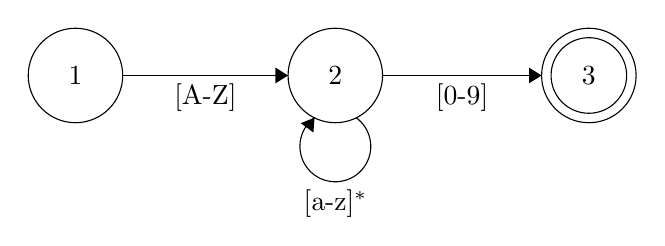
\begin{tikzpicture}[scale=0.2]
	\tikzstyle{every node}+=[inner sep=0pt]
	\draw [black] (22.9,-27) circle (3);
	\draw (22.9,-27) node {$1$};
	\draw [black] (39.4,-27) circle (3);
	\draw (39.4,-27) node {$2$};
	\draw [black] (55.5,-27) circle (3);
	\draw (55.5,-27) node {$3$};
	\draw [black] (55.5,-27) circle (2.4);
	\draw [black] (25.9,-27) -- (36.4,-27);
	\fill [black] (36.4,-27) -- (35.6,-26.5) -- (35.6,-27.5);
	\draw (31.15,-27.5) node [below] {[A-Z]};
	\draw [black] (42.4,-27) -- (52.5,-27);
	\fill [black] (52.5,-27) -- (51.7,-26.5) -- (51.7,-27.5);
	\draw (47.45,-27.5) node [below] {[0-9]};
	\draw [black] (40.723,-29.68) arc (54:-234:2.25);
	\draw (39.4,-34.25) node [below] {[a-z]$^*$};
	\fill [black] (38.08,-29.68) -- (37.2,-30.03) -- (38.01,-30.62);
	\end{tikzpicture}
\end{center}
\vspace{5mm}

Regular languages and, by extension, finite-state machines are often used in string searching algorithms. FSMs and regular languages are also often used in the lexical analysis (lexing) done by a compiler. That is, they give language designers the power to specify which words are valid in their programming language. \\

\subsubsection{Pushdown Automata}

Pushdown automata (PDA) are finite-state machines that also have access to a stack. These automata introduce a notion of \textit{history} or \textit{memory}. A PDA can push a symbol onto its stack on every transition, which will provide information in the future about actions in the past. It can also pop or peek at the stack to decide which transition to take next. \\

Pushdown automata can distinguish syntactically correct sentences from random sequences of valid words, something finite-state automata cannot do because they have no notion of what comes earlier than a given point in a given sentence. For example, a pushdown automaton would be able to tell that "my dog bites red toys" is a valid English sentence and "red my toys dog bites" is not. However, PDA cannot understand semantics. It would also consider "my dog \textit{barks} red toys" a valid English sentence, even though it has no meaning. \\

Pushdown automata can read \textit{context-free languages}, which are languages that follow a \textit{context-free grammar}. Context-free languages are formal languages whose production rules are of the form $A\rightarrow\alpha$ where $A$ is a nonterminal and $\alpha$ is a sequence that may contain terminals and nonterminals. A PDA pops terminals from its stack. When a nonterminal $A$ is at the top of the stack, the PDA can pop it and push the $\alpha$ of some production rule onto the stack. In a sense, the stack of the PDA contains the unprocessed data of the grammar. \\

Context-free grammars can be written to formalize languages such as the language of matching parentheses or the language of infix algebraic expressions (e.g. (2+4)/7*8). PDA and context-free languages are often used in the syntactic analysis (parsing) done by a compiler. That is, they give language designers the power to specify how valid sentences are structured in their programming language. \\

\subsubsection{Linear Bounded Automata}

Imagine that, instead of a stack, an automaton could have access to a finite-length list. Linear bounded automata (LBA) have a finite number of \textit{states}, a finite length of \textit{tape}, and a \textit{head} that can read and write symbols on the tape and move left or right along it, one symbol at a time. The length of the tape is a linear function of the length of the input, so we can say that the tape has $kn$ cells, where $n$ is the length of the input instructions and $k$ is a constant. \\

This machine is similar to the idea of a modern computer. The tape represents a finite amount of memory, and the head is able to read and write to it. LBA can understand \textit{context-sensitive languages}, which are languages that follow a \textit{context-sensitive grammar}. Sophisticated programming languages are context-sensitive, so a linear bounded automaton would be able to read and understand modern software. The $kn$-length tape acts as a sufficient environment for computationally demanding programming tasks, given a large enough $k$. Similarly, given enough memory, real computers can also solve very computationally difficult problems. \\

A context-sensitive language is a language where semantics matter. Using our earlier example, "my dog barks red toys" would not be a valid sentence in a context-sensitive version of English. An LBA then is actually able to differentiate data types and can tell when an operation is defined for one type and undefined for another. LBA and context-sensitive languages are often used in the semantic analysis (type checking) done by a compiler. That is, they give language designers the power to specify whether or not a syntactically correct sentence actually has any real \textit{meaning} in their programming language. \\

Where can we go from here? LBA are suitable models of real-world computers, and they can process semantic language. What more can we do? Let's try making the tape infinitely long$\dots$ \\

\subsubsection{Turing Machines}

A \textit{Turing machine} (TM) not only models real-world computers, but \textit{computation} itself. The concept, which was formalized in 1936 by Alan Turing, generalizes automata and defines the limitations of mechanical computing. It specifies a set of components that are necessary and sufficient for creating a "problem-solving machine" that is capable of solving any problem that can be solved by a machine. Weaker automata can solve \textit{some} of these machine-solvable problems, but only \textit{Turing-complete} automata (those that are functionally equivalent to TMs) have the expressive power to solve \textit{any} of them. The components of a Turing machine are listed below.

\begin{itemize}
\item An infinitely long \textit{tape} that is divided into cells, each of which contains a symbol from some finite alphabet. One symbol from this alphabet is considered blank, and the tape is initially filled with these symbols.
\item A \textit{head} that can read and write symbols on the tape and move left or right along it, one symbol at a time.
\item A \textit{state register} that stores its current state and initially stores its starting state.
\item A \textit{finite table of instructions} that, given the machine's current state and tape symbol, tells the machine to do the following sequence of actions:
	\begin{enumerate}
		\item Erase or write a symbol at the current tape cell (or do nothing)
		\item Move the head one tape cell to the left or right (or do nothing).
		\item Depending on the current state and input, transition to a different state (or the same state) or halt computation.
	\end{enumerate}
\end{itemize}

A machine like this need not be a real-world computer. In fact, in his original proof, \textit{On Computable Numbers, with an Application to the Entscheidungsproblem}, Turing refers to a person, whom he calls the "computer," as an example of a Turing machine. If we break down these components into the resources they represent, it becomes clear that many systems could be considered Turing machines.

\begin{itemize}
	\item The infinitely long tape represents \textit{infinite space for computation} or \textit{infinite memory}.
	\item The head represents three abilities:
		\begin{enumerate}
			\item Reading memory,
			\item Writing to memory,
			\item Traversing the memory freely, with no side effects.
		\end{enumerate}
	\item The state register represents the ability to \textit{know what "step" you are on} in the problem-solving process. We will clarify this ambiguous idea in a second, but for now just think of it as having an idea of your progress.
	\item The finite table of instructions represents a \textit{sequence of commands} or \textit{program} that can be followed unambiguously. The automaton can follow and obey these commands in order without any actual thought.
\end{itemize}

As long as you have unlimited space to work in, the freedom to read and write symbols anywhere in that space, a list of instructions to follow exactly, and the knowledge of what to do next, you have a Turing machine. We can now visualize the person Turing referred to as a "computer." It is a man with an infinitely large piece of paper, a pen that he writes symbols with, a list of instructions that tells him which symbols to write, where on the paper to move his pen tip, which instruction to perform next, and a knowledge of which instruction he is currently performing. Many systems of logic, such as programming languages, are Turing-complete. Many things not traditionally thought of as "systems of logic" are \hrefcolor[blue]{https://www.toothycat.net/~hologram/Turing/index.html}{\underline{also Turing-complete}}. \\\\

\begin{tcolorbox}[breakable, enhanced, colback=textbook-blue, sharp corners]
	\vspace{3mm}
	\begin{center}
		\textbf{Turing Machines and Consciousness}
	\end{center}
	In 1950, Turing developed the \textit{Turing test}, a test of a machine's ability to exhibit behavior indistinguishable from that of a human. It involves an interrogator who is tasked with having two separate text conversations and determining which of the two participants is actually a machine. If the interrogator cannot distinguish a difference, the machine has passed the test. Despite its importance to the philosophy of computer science, the test is not a good indicator of whether or not a computer can think. The test says more about how gullible the interrogator is than how conscious the computer is. At the end of the day, the computer is still following its programming. \\
	
	What about this man whom Turing calls a "computer"? Would he pass the test, given the right programming? Perhaps he would. But that would not make him a \textit{person}. What kind of person is this man if he follows whatever instructions he is given? He is a slave, a person who always obeys. Could we say then that machines are also, in a certain sense of the word, slaves? Perhaps this is where the term \textit{master-slave technology} came from. Regardless, it is important to make a philosophical distinction here about what separates humans from machines or, more precisely, what distinguishes \textit{thought} from \textit{computation}. \\
	
	Essentially, this boils down to the question of consciousness. There is much debate about consciousness. Philosophers have proposed a variety of concepts that partially define it such as free will (the ability to choose) or qualia (the raw experience of existence, e.g. sounds, colors, emotions). However, \textit{intentionality} is one characteristic that is generally agreed upon as necessary for conscious thought. Intentionality is the ability of the mind to think \textit{about} something. Computers can \textit{think} things, but they cannot \textit{think about} things. They lack intentionality.\\
	
	For a Turing machine, the list of instructions is an essential component. It is capable of "thinking" if and only if some one tells it what to think. That effort is more accurately defined by the term "computation." We would also refer to the man's efforts with his pen and infinite paper as computations because they require no thought. If he were nothing more than a Turing machine, the man would not be able to perform mathematics on his own. In fact, he would not be able to do anything without instructions. It is the moment when he does something without being explicitly told to do it that he first displays consciousness. When \textit{unprompted} computation is performed for some \textit{purpose}, we can talk about consciousness. \\
	
	So calling computers slaves is a bit of an anthropomorphization. A slave is a conscious being who is forced to act like a machine. Computers don't have the prerequisite consciousness. No matter how complicated its architecture or sophisticated its artificial intelligence software, a computer is a \textit{tool} like a microwave or a calculator. Could it ever be more than that? Could a technology ever think? \hrefcolor[blue]{https://en.wikipedia.org/wiki/Artificial\_consciousness}{\underline{Perhaps}}. But such a thing would be quite different from a Turing machine or any modern computer. \\
	
	\parbreak
	\vspace{1mm}
	
	\begin{displayquote}
		\textit{In attempting to construct such machines we should not be irreverently usurping His power of creating souls, any more than we are in the procreation of children: rather we are, in either case, instruments of His will providing mansions for the souls that He creates.}
		\vspace{4mm}
		\begin{flushright}
			---Alan Turing (1950), \\
			in response to a theological objection to artificial consciousness.
		\end{flushright}
	\end{displayquote}
	\vspace{3mm}
\end{tcolorbox}
\vspace{2\baselineskip}

A single-tape Turing machine is formally defined as a septuple $(Q,\Gamma,b,\Sigma,\delta,q_0,F)$, where

\begin{itemize}
	\item $Q$ is a finite, non-empty set of \textit{states},
	\item $\Gamma$ is a finite, non-empty \textit{tape alphabet},
	\item $b\in\Gamma$ is the \textit{blank symbol},
	\item $\Sigma\subseteq\Gamma\setminus \{b\}$ is the set of symbols that can be written on the tape,
	\item $\delta$ is a partial function $\delta : (Q\setminus F)\times\Gamma\nrightarrow \Gamma\times\{L,R\}\times Q$ called the \textit{transition function}, which inputs the current state and tape symbol and outputs the symbol to write to the tape, the direction to move the head, and the next state to transition to,
	\item $q_0\in Q$ is the \textit{starting state}, and
	\item $F\subseteq Q$ is the set of \textit{final states}. The contents of the tape are \textit{accepted} if the Turing machine halts computation in a state from $F$.
\end{itemize}

We should now address what exactly "state" is in regard to computing. Many people associate it with the current instruction being fed to the machine. However, Turing made a distinction between this interpretation of state and the interpretation of state as the computer's "progress" or "state of mind." Turing's \textit{complete configuration} of state includes not only the current instruction, but the current symbol configuration of the entire tape as well and all the instructions yet to be executed. In this way, state is defined by the results of past instructions and the inevitable execution of future instructions. \\

Now we have defined what a Turing machine is, but it is still not clear why it is considered such a landmark concept in computer science. For example, if real-world computers can be sufficiently modeled by linear bounded automata, why do we instead focus so heavily on Turing machines? \\

Turing machines are the class of automata that can read \textit{recursively enumerable languages}. A formal language is called recursively enumerable, if it is a \textit{recursively enumerable subset} in the set of all possible words over the alphabet of the language. This essentially means that, for a language of this type, there exists an algorithm that can output a list of every word in the language. Consider what would be required for such an algorithm. How many valid words are there in a given language? Depending on its rules for constructing words, there may be an infinite amount. This is the case for some programming languages. A variable name could theoretically be as long as you want, provided you have enough memory to store it. In order to list all of the words in a recursively enumerable language, you would need infinite memory, which only a Turing machine can provide. \\

This does not imply that TMs can handle infinite lists of instructions. Rather, they can handle \textit{infinite looping} over a finite set of instructions. A Turing machine can "successfully" run a never-ending program. A real machine would use up all of its memory trying to run such a program, eventually crashing due to a \textit{stack overflow} (an attempt to write data outside of the limits of the memory). A TM would never run out of memory and, given infinite time, could run the program forever. \\

As previously stated, the Turing machine models not only computers, but \textit{computation}. It abstracts away the physical limitations of computers such as memory constraints, overheating, or hardware failure and asks what the fundamental limits of algorithmic computation are. It makes a statement on which mathematical problems are \textit{decidable}. It is an ideal computer, and, as such, it is not only a model of what real-world computers are today, but a model of what they \textit{could be} in the future, given sufficient advances in hardware. \\

%----------------------------------------

\subsection{The Importance of Turing Machines to Modern Computing}

The automata we have discussed so far (finite-state machines, pushdown automata, linear bounded automata, and Turing machines) form a sort of hierarchy of machine capability. The formal grammars and languages that these automata can understand likewise constitute a hierarchy that was first described by Noam Chomsky in 1956. The \textit{Chomsky hierarchy}, a classification of the expressiveness of language according to grammatical rules, is summarized below by a table with columns for grammars, the languages those grammars build, and the class of automaton that can understand those languages.

\begin{table}[H]
	\caption{The Chomsky Hierarchy}
	\label{tab:LABEL}
	\begin{tabularx}{\textwidth}{|c|c|Y|}
		\vtabularspace{3}
		\hline
		Grammar & Language & Automaton \\
		\hline
		Type-0 & Recursively enumerable & Turing machine \\
		Type-1 & Context-sensitive & Linear bounded automaton \\
		Type-2 & Context-free & Pushdown automaton \\
		Type-3 & Regular & Finite-state machine \\
		\hline
		\vtabularspace{3}
	\end{tabularx}
\end{table}

As this is a hierarchy, higher-ranking automata are capable of doing anything that lower-ranking automata can. For example, an LBA can do anything that a PDA or FSM can and \textit{more}. To give a linguistic analogy, an LBA would be fluent in all of the languages that the PDA and FSM are fluent in, but would also be fluent in additional languages. What causes this difference in language facility? It is the structure of the automaton's memory. \\

Let's recap how these four automata handle memory.

\begin{itemize}
	\item An FSM has \textit{no} memory. It simply has a finite number of states, perhaps represented by a finite list of instructions. It can transition between states, but it has no notion of how it got to any particular state. It records no history.
	\item A PDA has a \textit{stack} of memory, but this form of memory is restricted. It cannot read or write its memory in any order it likes. It can read the top entry on the stack, but it must delete data to read entries located elsewhere.
	\item An LBA has a \textit{finite array} of memory. It can read or write this memory in any order it likes, but it has limitations on how much information it can store.
	\item A TM has an \textit{infinite array} of memory. It can read or write this memory in any order it likes, and it can also store as much as it likes.
\end{itemize}

It is no coincidence that real-world computers today use array-based memory. Arrays are both an intuitive and Turing-complete way to store information. Now, technically, LBA and TMs use "tape" instead of arrays, but the differences are minimal. In tape memory, cells have relative position, but they are not \textit{labeled}. Modern computers are actually modeled by \textit{register machines}. Register machines are equivalent in expressive power to Turing machines, but their memory is composed of an infinite-length array of uniquely addressed \textit{registers}. Like a tape of cells, an array of registers can be freely accessed. \\

A subset of register machines known as \textit{random-access machines} allow for \textsc{jump} instructions (e.g. jump to register \#5623) in addition to standard sequential traversal of memory (e.g. move right, move right, move right, etc). This allows computers to accomplish a task with fewer instructions, but the expressive powers of random-access machines and Turing machines are equivalent because both are capable of \textit{eventually} solving the task. Modern computers can be described as random-access machines because they use \textit{random-access memory} (RAM). In RAM, the time to access information is independent of physical location. From a performance perspective, this means that we do not have to consider \textit{where} we store things in memory. It's all uniformly fast. This allows for the construction of \textit{node-based} data structures, which we will discuss in a later section. \\\\

\begin{tcolorbox}[breakable, enhanced, colback=textbook-blue, sharp corners]
	
	\vspace{3mm}
	
	\begin{center}
		\textbf{Exploring Exotic Automata}
	\end{center}

	It is worth thinking about automata whose memory is modeled by non-list data structures. For example, a pushdown automaton uses a stack to model its memory and because of this, it is not Turing-complete. What if it used a queue instead? In this case, it would be Turing-complete because it could dequeue items to traverse the memory and then enqueue them to avoid data loss. One could envision this as a Turing machine whose infinite tape ends are glued together to form an infinite loop. The machine can only move in one direction, but it can still access every cell because its tape is circular. \\
	
	The memory can also be modeled by non-sequential data structures to create some bizarre models of computation. What if the memory of a computer was laid out not as an array, but as an undirected tree? What if it was organized according to an algebraic structure like a monoid or a ring? I'm not even going to pretend that I understand what kind of behavior this would result in. But it is an \hrefcolor[blue]{https://kluedo.ub.uni-kl.de/frontdoor/index/index/docId/4400}{\underline{area of active research}}. \\
	
	Other tweaks can be made to the properties of a Turing machine to create new, interesting automata. For example, \textit{$\omega$-automata} (or \textit{stream automata}) are Turing machines that expect an \textit{infinite} sequence of instructions. \textit{$\omega$-automata} never stop running because an infinite sequence of instructions requires an infinite sequence of instruction executions. Because they never terminate, they never move into acceptance (final) states. Rather than a set of final states $F$, they have a set of \textit{acceptance conditions} $Acc$. \\
	
	For ordinary automata, every \textit{run} $\rho$ (i.e. a sequence of $n$ states) ends with a state $r_n$, and the input is only accepted if this state is final (i.e. $r_n\in F$). For $\omega$-automata, runs are infinite sequences, so they do not end with a state $r_n$ at all. How do we tell if a run $\rho$ should be accepted as a valid set of instructions? We require that $\rho\in Acc$. That is, if the run is a member of the "set of acceptable runs," it should be accepted. What is the "set of acceptable runs"? That depends on which variant of $\omega$-automaton you are talking about. \\
	
	The class of $\omega$-automata contains multiple automata with different definitions of $Acc$. For example, for some subset $F$ (final states) of $Q$ (all states), the \textit{B\"{u}chi automaton} accepts those runs $\rho$, for which there exists a final state that occurs "infinitely often" in $\rho$. What is a state that is visited "infinitely often"? Given an infinite amount of runtime, some states in $Q$ will be visited an infinite amount of times, and others will not. For example, what if you can transition away from your starting state $q_0$, but you are not allowed to transition into it. Even given infinite time, $q_0$ would not be visited infinitely often, and if it were the only state in $F$, you would never be able to construct a run that would be considered valid by a B\"{u}chi automaton. Nondeterministic B\"{u}chi automata have applications in "always-on" or "always listening" software, such as those used in highly-autonomous robots or smart speakers like the Amazon Echo, both of which receive instructions based on a never-ending, real-time stream of sensory data. \\
	
	Wow, that's a lot of abstract mathematics. Why is any of this important for gaining a fundamental understanding of Turing machines or real-world computers? It is important because we can only really grasp their \textit{scope} if we explore outside of it. Some automata can have properties that are not practical or possible to implement in the real-world. Mathematically, they could have infinite states or continuous alphabets or hyperdimensional memory. But here, once and for all, let's define the scope of computation we will be considering for the rest of this guide. \\
	
	A modern computer has:
	
	\begin{itemize}
		\item A \textbf{finite} set of states Q. If it were instead infinite, the automaton would have a state for every possible input, and thus would be able to understand any conceivable language. This is far too powerful a machine to build. This would essentially be a universal problem solver.
		\item A \textbf{finite} alphabet $\Sigma$. If it were instead infinite, the automaton could have a continuous alphabet. What kind of alphabet's symbols exist on a spectrum? Perhaps you could call \textit{sound} a "language" with a continuous alphabet known as frequency. An automaton with an infinite alphabet would not be digital and would not use bits. It would be an analog computer. Analog computers do exist, and they were popular in the 1950s and 1960s, but nowadays we write software for digital computers. \textit{Fun fact:} analog synthesizers, which are still commonly used in electronic music, are considered a kind of analog computer.
		\item A transition \textbf{function} $\delta$. If it were instead a relation (i.e. inputs are mapped to more than one output), the automaton would be nondeterministic. It is suspected that nondeterministic Turing machines would be able to solve NP-complete problems, which is a computational feat that has not yet been accomplished in a tractable way by a deterministic Turing machine.
	\end{itemize}

	\vspace{3mm}
	
\end{tcolorbox}
\vspace{2\baselineskip}

While more exotic memory structures are theoretically possible, real-world computers use \textit{arrays} of memory. Since Turing machines can solve any computable problem and data structures are used by computers to solve problems, it follows that data structures can be simulated by Turing machines. Because register machines use array-based memory and are Turing-equivalent, it also follows that \textbf{all data structures can be implemented using arrays}. This is a very useful insight, and it will be discussed further in Section 3. \\

The selection of Turing machines (or register machines) as the model for real-world computers has also influenced decisions in computer architecture. In early computers, the instructions were not integrated into the machine. Code was written on punch cards, which were fed into computers. Eventually, code was stored digitally in programs that were uploaded to the computer's memory. This type of machine is known as a \textit{stored-program computer}. \\

Where should one store instructions or code in a stored-program computer? Those that have a \textit{Harvard architecture} store their instructions in an \textit{instruction memory} that is separate from the \textit{data memory}. Those that have a \textit{von Neumann architecture} store their instructions and data in the same physical memory, but partition the memory somehow to avoid overwriting the instructions. The von Neumann architecture allows "programs that write programs," such as assemblers, compilers, linkers, and loaders. Modern computers are more von Neumann than they are Harvard because their instructions and data share an address space, but they are not strictly either. We can describe modern computers as \textit{random-access stored-program} (RASP) machines with \textit{split-cache modified Harvard architectures}. \\

%----------------------------------------

\subsection{Modern Hardware Implementation}

% We've discussed "computers" in many different ways (primitive examples, pre-Turing examples, theoretically).
% The typical modern computer is programmable (in a Turing-complete sense), digital, electronic, stored-program, general-purpose, uses RAM, uses so-and-so architecture
% Maybe some ubiquituous devices and "optional" components (like hard drives and I/O)
% Maybe discuss some important non-standard computers (embedded systems, datacenters, supercomputers).

% Signals, clock cycles
% Byte vs word addressing
	
%--------------------------------------------------------------------------------
%    SECTION: COMPUTABILITY THEORY
%--------------------------------------------------------------------------------

\toclineskip
\section{Computability Theory}

\vspace{4mm}
\begin{displayquote}
\textit{Thirty years ago, we used to ask: Can a computer simulate all processes of logic? The answer was yes, but the question was surely wrong. We should have asked: Can logic simulate all sequences of cause and effect? And the answer would have been no.}
\begin{flushright}
	---Gregory Bateson
\end{flushright}
\end{displayquote}
\vspace{4mm}

% Rewrite at the end

Computation is mathematical in nature. Underneath its shiny UI and immersive applications, a computer is simply a machine that can be programmed to calculate numbers (and do it \textit{very} quickly in the case of modern computers). With that said, let me pose the central question of computability theory: could a machine (or computer) theoretically solve any given math problem, if given the correct input (or code)? We will consider this question more formally in this section, but it turns out that the answer is no. There exist problems that a computer will never be able to solve with computation, even given infinite resources. \\

In this section, we will discuss what makes a problem \textit{solvable} and thus within the scope of computational analysis. We will also briefly discuss \textit{unsolvable} problems and how they can be organized into a hierarchy of \textit{unsolvability}. That said, before we discuss either solvable or unsolvable problems, we need to formalize our definition of the term \textit{problem} with regard to the field of computer science. \\

%----------------------------------------

\subsection{The Scope of Problem Solving}

% Rewrite -- what are problems, why are they worth solving, what is calculation, what is computation?

% Domains of discourse / universes in classical logic are just types in type theory. Top = true in every universe, Bottom = true in no universes (false)

% Use sequent notation to explain axioms
% Formal systems
% Proof calculi (Hilbert)
% Automata are formal systems

Since computation is mathematical, it follows that the natural use of computers is to solve \textit{mathematical problems}. A mathematical problem is a problem that is amenable to being represented with mathematics. Are there problems that are not mathematical? That is, are there problems that either \textit{cannot} be formalized with mathematics or \textit{should not} be formalized with mathematics because the result would produce no valuable insight? Of course. You might say that certain "human" problems are not mathematical in nature. For example, can an ethical problem be solved \textit{mathematically}? Furthermore, what does it mean for a problem to have a mathematical solution? It turns out that the answer lies in the difference between \textit{reasoning} and \textit{logic}. \\

% Curry-Howard: proofs and programs are the same thing. 

% A deductive system is a "calculus"
% Argument - set of statements (premises) and a conclusion in a language
% Premises can be axioms or theorems
% Logical consequence
% Truth-bearer
% Deductive reasoning is applied to an argument to create a deduction (argument + steps of reasoning)
% Composing a deduction is a way to prove validity
% Composing an induction is a way to assess strength
% Venn diagrams
% Reasoning is a set of rules of inference
% Inductive/deductive "steps"
% Proof - deduction from "known truths" (axioms and proven theorems), proves soundness
% Data validation proves cogency?
% Argument vs explanation
% Validity/soundness

\subsubsection{Informal Logic}

% Discuss the logical reasonings comparatively. 3 paths in life. Certain vs uncertain. Binary vs multi-valued.

% Interlocuters
% Fallacious reasoning
% Formal vs informal (indep of interpretation)

\subsubsection{Formal Logic}

% Common logical symbols wiki
% Domain of discourse / universe
% Deduction is impossible in non-axiomatic systems because we don't know what the axioms of the Universe are.

% What is logic?
Logic is a long-standing, far-reaching field, and its definition has changed over the ages, but it can be broadly described as the study of \textit{argument}. 

% What is early logic?
The practice and analysis of logic can be done in many different ways. For example, the early study of logic was mostly done in the context of \textit{natural language} arguments made during oration.

% Syllogistic logic (categorical reasoning, motivated by science 13:45)
% Stoic logic

% Informal logic is not always explicit. It may have implicit elements that must be made explicit by analysis.
% Formal logic, traditionally symbolic logic, now called mathematical logic

% What is modern logic? ("Arguments and the forms they make take")
Modern logic, however, is \textit{formal}. That is, it observes the abstract \textit{forms} of arguments instead of the arguments themselves. \\

% Hobbes - thought as computation
% Boolean logic
% Frege, logicism
% Class - Russell's paradox

Formal logic is the study of \textit{inference} with regard to \textit{formul{\ae}}. Formul{\ae}, Latin for "small forms" or "small rules," are finite sequences of symbols from an alphabet. They are purely \textit{syntactic objects}, much like strings of text. Inference is the act of processing a formula $A$ and deducing that a formula $B$ is a \textit{logical consequence} of $A$. This means that, given a set of \textit{rules of inference}, the string $A$ can be transformed into the string $B$ by means of a finite series of applications of said rules. \\


% Logical and non-logical symbols
% Categorematic and syncategorematic terms (individual meaning)
% Formal systems
% Reason vs. logic -> Humans vs. computers
% Model theory

% Set theory is intertwined with two-valued logic via the membership function

% Fuzzy set theory
% Membership functions between 0 and 1

and they are studied in within \textit{formal systems}. These systems of abstract thoughts are used to infer the existence of formul{\ae} by means of logical deduction starting from a given set of axioms. A formal system has:

\begin{enumerate}
	\item A finite \textit{alphabet} of \textit{symbols}, from which a formula may be constructed
	\item A formal \textit{grammar}, to which a formula must conform if it is to be considered \textit{well-formed} in the system
	\item A set of initial formul{\ae}, known as \textit{axioms}, from which inferences can be made
	\item A set of inference rules, known as a \textit{logical calculus}, which prescribe how inferences are to be made
\end{enumerate}

%%%

Formul{\ae}, which are finite sequences of symbols from a system's alphabet, are purely \textit{syntactic} objects, but, given an \textit{interpretation}, they can be endowed with \textit{semantic} meaning. For example, an interpretation of first-order logic requires the following assignments of semantic meaning:

\begin{enumerate}
	\item Variables are assigned \textit{objects} (things that can be modeled) from a \textit{domain of discourse} (a well-defined set of objects)
	\item Predicates are assigned \textit{properties} of objects
	\item Formul{\ae}, which contain variables and predicates, are assigned a \textit{truth value} of true or false
\end{enumerate}

A well-formed formula with such an interpretation is called a \textit{sentence}, and the meaning expressed by a sentence is called a \textit{statement} or \textit{proposition}. A sentence expressing a true statement (according to the axioms and inference rules of the formal system) is called a \textit{theorem}, and a set of theorems is called a \textit{theory}. For example, ZFC set theory is a first-order \textit{theory} of sets. It has a collection of theorems written in first-order logic that form an \textit{axiomatic set}, and these theorems are used to prove other theorems that also belong to the theory using a set of inference rules. \\

\subsubsection{Decision Problems and Function Problems}

First-order logic is also called \textit{predicate calculus}. It is a system for calculating \textit{predicates}, which are Boolean-valued functions. In mathematics, a predicate maps \textit{propositions} written in first-order logic to Boolean values (i.e. $P:X\rightarrow \{\textsc{true},\textsc{false}\}$). In linguistics, a proposition can be written in the form of a \textit{yes-no question} without sacrificing any semantic meaning. For example, evaluating the proposition "The sky is blue." as true or false is the same thing as answering the question "Is the sky blue?" with either yes or no. \\

More generally, a predicate is a function that receives an input and makes a binary decision about it. In computability theory, the analogous concept is called a \textit{decision problem}, a problem that can be posed as a yes-no question. Decision problems are fundamental to mathematical practice. A proof of a mathematical statement is a decision problem. Additionally, formal verification of a proof involves solving a series of decision problems regarding whether or not each statement in the proof can be reduced to its axioms. The proof is valid if and only if all of its statements are. Decision problems are problems that can be solved by \textit{making a decision} (mapping the question to a yes-no answer).  \\

It is natural to expect that computers, which are tools for doing math, should be able to solve decision problems. That said, computers can handle more than just Boolean-valued functions. They can represent functions of \textit{arbitrary} return type (e.g. integers, words, objects, etc.). This allows them to solve the broader class of \textit{function problems}, problems where a single output is expected for every valid input. Function problems are problems that can be solved by \textit{calculating a function} (mapping the problem input to a solution output). \\

One important example of a decision problem is whether or not a given function problem is solvable. Let $F$ be a \textit{function problem}, and let $D$ be the \textit{decision problem} of whether or not $F$ is solvable for each of its inputs. Let $f:X\rightarrow Y$ be a \textit{function} that solves $F$, where $X$ is the set of all problem inputs and $Y$ is the set of all problem outputs. Let $G(f)$ denote the set of all ordered pairs $(x,f(x))$ such that $x\in X$. $G(f)$ is known as the \textit{graph} of the function $f$. Let $d:X\rightarrow \{\textsc{true},\textsc{false}\}$ be a decision that solves $D$. For each $x\in X$, $d(x)$ is $\textsc{true}$ if and only if there exists an ordered pair $(x,f(x))$ in $G(f)$. Otherwise, $d(x)$ is $\textsc{false}$. \\

Here's a more concrete example. Let $x$ be any natural number (including 0). $F$ asks "What is $\rfrac{2}{x}$ for all $x$?." $D$ asks "Does $\rfrac{2}{x}$ exist for all $x$?." In both cases, $f(x)=\rfrac{2}{x}$, but $F$ is interested in the \textit{value} of each of the outputs while $D$ is interested in the \textit{existence} of each of the outputs. There is one input for which $f$ has no defined output and that is $x=0$. In this case, the answer to $D$ is negative, and $F$ is technically unsolvable. That said, we can just move the goalposts a little bit to make $F$ solvable by allowing $f$ to be a partial function: $f:\mathbb{N}\nrightarrow \mathbb{N}$. Partial functions do not necessarily map every member of their domain to a value. Thus, they can be \textit{undefined} for some input values. As long as "undefined" is considered a valid answer to $F$, $F$ can be considered solvable for its whole domain. \\

In computability theory, we are interested in determining whether or not an output exists for each of a problem's inputs. If an output exists, we can be sure it has \textit{a} value, but the particular value is inconsequential. While computers do solve function problems, it is enough to consider only the corresponding decision problem when proving whether a function problem is \textit{solvable} or not. \\

\subsubsection{"Effective Calculability"}

Before the study of computer science, mathematicians sometimes informally described functions as \textit{effectively calculable}. This meant that a correct output could be calculated for any input from the domain of the function, using an \textit{effective method}. A method, in general, is just a "procedure" that does "something." A method is \textit{effective} if it consists of a finite number of instructions and solves a particular problem. \\

A particular method can be effective for some problems and ineffective for others. For example, typing is a method. If I want to put characters into a text document, typing is an effective method. If I want to plant a flower, typing is not an effective method. However, if I want to plant a flower, building a flower-planting robot and programming it, via typing, to plant a flower \textit{is} an effective method because it actually accomplishes the objective. An effective method that is used to calculate the values of a function is called an \textit{algorithm}. \\

Much work was done in the 1930s to formalize "effective calculability." The results established \textit{Turing computability} as the correct formalization. This model gives the following fundamental definition: any function whose outputs can be calculated by an algorithm is a \textit{computable function}. Computable functions are precisely those functions that can be computed by a Turing machine. In the mathematical sense, they could also be called \textit{solvable}. A computable or solvable \textit{decision} is predictably called \textit{decidable}. If the functions model mathematical proofs, they could also be called \textit{provable}. Despite a few minor differences, all of these terms get at the same idea. \\

We will now discuss the history preceding and the circumstances of this foundational work in formalizing "effective calculability" as computability. Much of this work was done between the 1930s and the 1950s, but it built heavily on set-theoretical concepts discovered by German mathematician Georg Cantor in the late 19th century. After a crash course in Cantorian set theory, we will examine computable functions from a variety of angles. Computability is interdisciplinary. The concept \textit{permeates} our reality, and as such its eventual formalization was made possibly by the collective efforts of mathematicians, logicians, linguists, and computer scientists. Today, research on computability is widespread in the study of anything scientific. \\

After a rigorous study of what is computable, we will conclude this section with a brief exploration of what is not computable. This is a topic that is important to theoretical computer science. By assuming that certain aspects of an abstract machine are \textit{hypercomputational}, we can envision the kind of problems that could be solved if computation were ever to transcend Turing machines. \\

%----------------------------------------

\subsection{The Ballad of Georg Cantor}

Georg Cantor (1845-1918) was a German mathematician whose work established \textit{set theory}, a fundamental theory in mathematics. Much of his work was built on generalizations of the set of natural numbers, namely the \textit{ordinal numbers} and the \textit{cardinal numbers}. These sets include both finite and \textit{infinite} quantities, a concept that was considered very controversial in the late 19th century. Despite an extreme amount of backlash, Cantor stood by his set theory and formalized what has been called "the first truly original idea in mathematics since those of the Greeks." \\

% Introduce the problem of the "size" of infinity.
% Example of the unit circle. The unit circle has a circumference of $2\pi$. It has circumference values of $[0,2\pi]\in\mathbb{R}$. Another way of saying this is that it has \textit{central angle} values of $[0,2\pi]\in\mathbb{R}$. The difference between that and, say, $a_n=\frac{1}{4}*n, n=[0,7]\in\mathbb{Z}$ is that all real intervals have an infinite number of possible values. But what happens when you go past 2\pi, \textit{beyond infinity}. You expand the infinite interval\dots to a another infinite interval. You'd be hard-pressed to find someone who argues that the interval $[0,4\pi]$ is \textit{not} bigger than $[0,2\pi]$. And yet, the intervals have the same "density" (they both have an infinite number of values). So the space doubled, and the density remained the same. This is not familiar to us. "Size" (number of elements) is not a useful measure of infinite sets. We need to generalize to cardinality.
% Are there infinite sets of different cardinalities? What if you doubled your interval an infinite amount of times?

\subsubsection{The First Article on Set Theory}

Cantor began his work in number theory, until his mentor, Leopold Kronecker, suggested that he answer an open question in real analysis: "If a given function can be represented by a trigonometric series, is that representation unique?." A trigonometric series is a series of the form
\begin{align*}
\frac{A_0}{2}+\sum_{n=1}^{\infty}(A_n\cos nx + B_n\sin nx).
\end{align*}
One common example of a trigonometric series is a Fourier series, which has coefficients $A_n$ and $B_n$ of the form
\begin{align*}
A_n&=\frac{1}{\pi}\int_{0}^{2\pi}f(x)\cos nx\,dx, \\[1mm]
B_n&=\frac{1}{\pi}\int_{0}^{2\pi}f(x)\sin nx\,dx,
\end{align*}
where $f$ is an integrable function. That said, Cantor's work concerned the general definition of a trigonometric series. He proved that any countable, closed set of natural numbers could encode a trigonometric series that uniquely represents a function. The qualifiers \textit{countable} and \textit{closed} are significant. A countable set is a set whose elements can be counted or enumerated. A closed set is a set that contains its limit points. For a trigonometric series, this means the set of all $n$ must contain a countable number of elements, two of which must be $1$ and $\infty$. $1$ is no problem, but what does it mean for a set to contain $\infty$? And, for example, how can the natural numbers between and including $1$ and $\infty$ be "countable"? \\

The concept of infinity had been around for a long time by the 1870s, but it had, until this point, been considered a philosophical topic. Aristotle identified a dichotomy between the "potential infinite" and the "actual infinite" in which the former can always have elements added to it while the latter is instead considered "complete." This mindset persisted for around two-thousand years with the majority of scholars believing that "actual infinity" was outside of the purview of mathematics. It was used in mathematical practice, but only in a non-rigorous, conceptual way, as seen in the characterization of limits "tending toward infinity." Actual infinity was considered an "ideal entity," not something that could be studied like finite numbers. \\

Here, however, Cantor had found a rigorous mathematical object containing infinity as an actual numerical quantity. If a set could represent a countable number of terms in a trigonometric series and was closed on $[1,\infty]$, it could look like $\{1,2,3,\dots,\infty\}$. It was this discovery that caused Cantor to think about the differences between a set like this, and a set like the real numbers, which, in addition to these values, could contain many more. He published his first article on set theory in 1874, stating two theorems that ushered in a new epoch of mathematical thought. \\

Cantor's first theorem from his 1874 article states that the set of real algebraic numbers can be put into one-to-one correspondence with the set of positive integers. An \textit{algebraic number} is any complex number that is a root of a non-zero polynomial with rational coefficients. That is, it is any $x\in\mathbb{C}$ that satisfies the following equation:
\begin{align*}
a_nx^n+a_{n-1}x^{n-1}+\cdots+a_2x^2+a_1x+a_0=0,
\end{align*}
where $a_0,\dots,a_n\in\mathbb{Q}$, at least one of which must be non-zero. A \textit{real algebraic number} or \textit{algebraic real} is then, logically, any algebraic number with an imaginary part of $0$. Complementary to the algebraic numbers are the \textit{transcendental numbers}, the real or complex numbers that are \textit{not} roots of any such polynomials, such as $\pi$ or $e$. \\

Cantor is stating here then that there exists a \textit{one-to-one correspondence} or \textit{bijection} between these algebraic reals and the positive integers (also known as the \textit{natural} or \textit{counting} numbers). An intuitive example of a bijection occurs when you touch the fingertips of your left hand to those of your right hand. Each left fingertip is paired with exactly one right fingertip, and vice versa. No fingertip is left unpaired. With this theorem, Cantor proves that the algebraic reals and the naturals are like the left and right hand. When paired one-to-one, no number from either set is left unpaired. \\

This discovery is almost unbelievable, and it is totally foreign to anything in finite mathematics. To put this into perspective, consider the fact that the algebraic reals contain the rational numbers. One would think that there would be far more rational numbers than positive integers, but when discussing infinite sets, it turns out that that is not the case. The rationals $\mathbb{Q}$, algebraic reals $\mathbb{A}_\mathbb{R}$, integers $\mathbb{Z}$, and naturals $\mathbb{N}$ are all examples of \textit{countably infinite} sets. That is, all of their elements can be put into a \textit{list}. While it may be difficult to see this quality in the rational numbers, it is made easier when you consider that the rational numbers are also called the \textit{measuring} numbers. While there are an infinite number of positive fractional measurements you could make while woodworking or cooking, these measurements can also be listed:
\begin{align*}
\Bigg\{\underbracket[0.25mm][2mm]{\frac{0}{1}}_0,\;\underbracket[0.25mm][2mm]{\frac{1}{1}}_1,\;\underbracket[0.25mm][2mm]{\frac{1}{2},\;\frac{2}{1}}_2,\;\underbracket[0.25mm][2mm]{\frac{1}{3},\;\frac{2}{3},\;\frac{3}{1},\;\frac{3}{2}}_3,\;\underbracket[0.25mm][2mm]{\frac{1}{4},\;\frac{3}{4},\;\frac{4}{1},\;\frac{4}{3}}_4,\;\underbracket[0.25mm][2mm]{\frac{1}{5},\;\frac{2}{5},\;\frac{3}{5},\;\frac{4}{5},\;\frac{5}{1},\;\frac{5}{2},\;\frac{5}{3},\;\frac{5}{4}}_5,\;\underbracket[0.25mm][4.4mm]{\cdots}_n\Bigg\}
\end{align*}
Note that each bracket has a number $n$ associated with it. Starting with $n=1$, the numbers in each bracket begin with $\rfrac{1}{n}$ and the numerator is incremented until you reach $\rfrac{n}{n}$. Then, you continue with $\rfrac{n}{1}$, incrementing the denominator until you reach $\rfrac{n}{n}$ again. Fractions whose values are already in the list are skipped. Negative rational numbers can be added by simply placing a number's complement immediately after itself in the list. Thus, $\mathbb{Q}$ is enumerable and countably infinite. \\

In his second theorem from his 1874 article, Cantor states that, given any sequence of real numbers $x_1,\,x_2,\,x_3,\,\dots$ in a closed interval $[a,b]$, there exists a number in $[a,b]$ that is not contained in the given sequence. Essentially, this means that, unlike the sets we just discussed, the set of real numbers $\mathbb{R}$ is \textit{not} enumerable or countably infinite. It cannot be expressed as a list or sequence because there will always be a real number missing. There exists no proper way to "count" the reals. With these two theorems, Cantor discovered that differences can exist between infinite sets. There are \textit{distinct} infinities. He comments on this in the same article: \\

\begin{displayquote}
	\textit{I have found the clear difference between a so-called continuum and a collection like the totality of real algebraic numbers.}
	\vspace{4mm}
\end{displayquote}

The truth of this "so-called continuum" of the real numbers would continue to evade Cantor for the rest of his life. In the years following his first article of set theory, he made a number of foundational discoveries related to this territory he termed the \textit{transfinite}. He began looking for a bijection between the unit line segment $[0,1]\in\mathbb{R}$ and the unit square (i.e. a square with sides of length $1$). In 1877, in a letter to his friend Richard Dedekind (of \textit{Dedekind cuts} fame), Cantor instead wrote a proof for the existence of a bijection between the unit line and all of the points in an $n$-dimensional space. Not only could the real numbers between $0$ and $1$ map \textit{one-to-one} with those in a $1\times1$ grid, they could map to all of the points in the plane, all of the points in 3-dimensional space, and all of the points in \textit{any} arbitrary dimension. Such was the nature of uncountably infinite sets. Cantor wrote to Dedekind below his proof: "I see it, but I don't believe it!" \\

\subsubsection{Ordinals and Cardinals}

To aid his exploration into the continuous nature of the real numbers, he formulated the \textit{transfinite arithmetic}, the arithmetic of infinite numbers whose size is somewhere between finite and uncountably infinite. He generalized the natural numbers, introducing two countably infinite sets, those of the \textit{ordinal} and \textit{cardinal} numbers. \\

Ordinal numbers describe order in a collection. More specifically, they describe the \textit{ordinality} of a number in an ordered set (e.g. $1^\textit{st}$, $2^\textit{nd}$, $3^\textit{rd}$, $\dots$). They include both finite natural numbers such as $1,\,2,\,3,\,\dots$ and transfinite numbers such as
\begin{align*}
\omega,\,\omega+1,\,\omega+2,\,\dots,\,2\omega,\,3\omega,\,4\omega,\,\dots,\,\omega^2,\,\omega^3,\,\omega^4,\,\dots,\,\omega^\omega,\,\omega^{\omega^\omega},\,\omega^{\omega^{\omega^\omega}},\,\dots
\end{align*}
where $\omega$ is the "first infinite ordinal." Note that this sequence of transfinite quantities never ends. Cantor commented on this property, stating that the set of all ordinals $\Omega$ cannot have a greatest member. Because $\Omega$ is well-ordered, there must exist some number $\delta$ that would be greater than all of the numbers in $\Omega$. But $\delta$ would belong to $\Omega$ because $\Omega$ contains all ordinal numbers. This implies that $\delta>\delta$, which is a contradiction. Cantor, a devout Lutheran, called this illusive $\Omega$ the Absolute Infinite, a number or set that is bigger than any conceivable quantity, finite or transfinite. This kind of thinking later led to the discovery of a number of \textit{mathematical paradoxes} or \textit{contradictions} in set theory, many of which still exist today. \\

Cardinal numbers describe the size or \textit{cardinality} of a set (i.e. a set could contain $1$ element, $2$ elements, $3$ elements, $\dots$). Like the ordinals, the cardinals include both finite natural numbers and transfinite numbers, the smallest of which is $\aleph_0$ (aleph-null). $\aleph_0$ is the cardinality of any countably infinite set, such as the natural numbers. In contrast to this, Cantor describes uncountably infinite sets, such as the real numbers, as having cardinality $\aleph_1$ (aleph-one). There are other greater aleph numbers that are studied for their own sake such as $\aleph_\omega$, the first uncountable cardinal number \textit{not} equal to $\aleph_1$. That said, $\aleph_0$ and $\aleph_1$ are sufficient for our purposes. Like the set of all ordinal numbers, the set of all cardinal numbers cannot be completed in any meaningful way and thus it can be described as a set of Absolute Infinite cardinality. \\

\subsubsection{The Continuum Hypothesis}

For much of his career, Cantor tried to prove the \textit{continuum hypothesis}, which states that there is no set whose cardinality is strictly between that of the integers and the real numbers. This would imply that there is no cardinal number between $\aleph_0$ and $\aleph_1$. If this hypothesis were true, the cardinality of $\mathbb{R}$ ($\aleph_1$) would be equal to the \textit{cardinality of the continuum} $\mathfrak{c}$ (a "continuum" being a set whose numbers "blend" into each other seamlessly). \\

To prove that $\mathfrak{c}=\aleph_1$, Cantor sought to relate $\mathfrak{c}$ to $\aleph_0$, and in doing so, he formulated a concept that is very relevant to combinatorics. He defined the \textit{power set operator} $\mathcal{P}$, which maps any set $S$ to its \textit{power set} $\mathcal{P}(S)$, the set of all subsets of $S$. For example, for a set $S=\{1,2,3\}$, $\mathcal{P}(S)$ contains the following sets:
\begin{align*}
\{\}\qquad\{1\}\qquad\{2\}\qquad\{3\}\qquad\{1,2\}\qquad\{1,3\}\qquad\{2,3\}\qquad\{1,2,3\}
\end{align*}
Notice that $S$ has cardinality $3$ and that $\mathcal{P}(S)$ has cardinality $2^3=8$. For any set $S$ with cardinality $x$, $\mathcal{P}(S)$ has cardinality $2^x$, and it turns out that this holds for transfinite cardinals as well. Thus, $\mathcal{P}(\mathbb{Z})=2^{\aleph_0}$. This expression is denoted with the character $\beth_1$ (beth-one) according to the following rule: $\beth_{\alpha+1}=2^{\aleph_\alpha}$. By \textit{Cantor's theorem}, $\beth_1 > \aleph_0$, so we can define $\mathfrak{c}=2^{\aleph_0}=\beth_1$ and state that $\mathfrak{c} > \aleph_0$. The continuum has a greater cardinality than a discrete set like the integers. The question then becomes: Could $\mathfrak{c}$ be anything less than $\aleph_1$, the cardinality of the real numbers? Or is the set of real numbers the smallest example of a continuum? \\

With the work of Kurt G\"odel in 1940 and of Paul Cohen in 1963, it was established that the continuum hypothesis cannot be proven or disproven. It is \textit{independent} of the axioms of Cantor's set theory. It is also independent of the axioms of the current foundation of mathematics, the \textit{Zermelo-Fraenkel set theory with the axiom of choice} (ZFC set theory). That said, since set theory works regardless of whether or not the continuum hypothesis is true, most mathematicians operate assuming that it \textit{is} true because the set of real numbers does appear to exhibit the behavior we would expect from a "continuum." Thus, independent of any particular set theory, we may assume that, for any transfinite cardinal $\lambda$, there is no cardinal $\kappa$ such that $\lambda<\kappa<2^\lambda$. \\\\

\begin{tcolorbox}[breakable, enhanced, colback=textbook-blue, sharp corners]
	\vspace{3mm}
	\begin{center}
		\textbf{Backlash Against Cantor's Set Theory}
	\end{center}
	Typically, when a proof is submitted, it is either quickly accepted by the mathematical community or quickly shown to be flawed. In the case of Georg Cantor's set theory, controversy loomed for many decades and objections came from many different angles. Most of the grievances came from the \textit{constructivists}, a group that was partially founded by Cantor's mentor, Leopold Kronecker. \\
	
	Constructivism is a \textit{philosophy of mathematics} that asserts that it is necessary to find or \textit{construct} a mathematical object in order to prove that it exists. Unlike \textit{classical mathematics}, \textit{constructive mathematics} does not adhere to the \textit{law of the excluded middle}, which states that a well-formed proposition must be either true or false. According to this philosophy, a \textit{proof by contradiction} (a proof of an object's existence founded in disproving the object's non-existence) is invalid. Constructivists took issue with the characterization of \textit{actual infinities} (e.g. the uncountably infinite set $\mathbb{R}$) as legitimate mathematical objects worthy of study. Their mathematical philosophy only permitted the existence of \textit{potential infinities} (e.g. the countably infinite set $\mathbb{N}$). Kronecker did not consider Cantor's original 1874 proof of a difference in cardinality between $\mathbb{N}$ and $\mathbb{R}$ as constructive. He remained staunchly opposed to Cantorian set theory and its hierarchy of the infinite, stating that \\
	
	\begin{center}
		\begin{displayquote}
			\centering
			\textit{God created the natural numbers; all else is the work of man.}
			\vspace{4mm}
		\end{displayquote}
	\end{center}

	There were other mathematical objections to Cantor's findings, such as those directed toward the uncountability of the transcendental numbers. By 1874, only a handful of transcendentals had been discovered. The constant $e$ was proven to be transcendental the year prior, and $\pi$ would not be proven to be transcendental until 1882. In stating that the algebraic reals were countable and the reals were not, Cantor implied that \textit{almost all} real numbers were transcendental. That is, if you remove a countable subset ($\mathbb{A}_\mathbb{R}$) from an uncountable set ($\mathbb{R}$), you are left with an uncountable subset ($\mathbb{A}_\mathbb{R}^c$, the \textit{complement} of the algebraic reals, also known as the transcendental reals). Many could not accept that something previously thought to be incredibly rare had instead an uncountably infinite number of examples. Other mathematicians, including Kronecker, refused even to accept Cantor's work as mathematical in nature, believing it to be, at best, philosophical. \\
	
	In addition to objections from mathematicians, Cantor's set theory received a number of complaints from Christian theologians. Some saw the formalization of an uncountable infinity as a challenge to the uniqueness of the absolute infinity of God. Some associated the transfinite hierarchy with pantheism. Cantor felt strongly that his set theory could exist harmoniously within a Christian framework. Even his notational choices ($\aleph$, $\omega$, and $\Omega$) can be considered an homage to the title of "Alpha and Omega." He associated the Absolute Infinite with God, and felt that transfinite quantities, while infinite, were no challenge to the supremacy of the Lord, averring that \\
	
	\begin{displayquote}
		$\dots$\textit{the transfinite species are just as much at the disposal of the intentions of the Creator and His absolute boundless will as are the finite numbers.}
	\end{displayquote}
	\vspace{4mm}
	
	Furthermore, Cantor wrote to numerous prominent theologians, including the Pope, in an attempt to clear up this confusion between the abstract notion of infinity and the actuality of infinity, as he saw it, in God and in Nature: \\
	
	\begin{displayquote}
		\textit{The actual infinite was distinguished by three relations: first, as it is realized in the supreme perfection, in the completely independent, extraworldly existence, in Deo, where I call it absolute infinite or simply absolute; second to the extent that it is represented in the dependent, creatural world; third as it can be conceived in abstracto in thought as a mathematical magnitude, number or ordertype. In the latter two relations, where it obviously reveals itself as limited and capable for further proliferation and hence familiar to the finite, I call it Transfinitum and strongly contrast it with the absolute.}
		\vspace{4mm}
	\end{displayquote}

	The onslaught of criticism began to wear Cantor down. Frustrated with the disapproval from his mentor and high-ranking members of his faith and with his inability to solve the continuum hypothesis, he fell into a chronic depression that persisted until his death. He ceased mathematical study for years at a time, writing and lecturing instead on Shakespeare. Nevertheless, some mathematicians, such as David Hilbert, supported his set theory. \\
	
	Hilbert championed the \textit{transfinitist} philosophy, which claims that infinite sets are legitimate mathematical objects. He believed that Cantor's set theory was the key to axiomatizing all of mathematics, a goal that he would pursue for much of his life. He gave lectures on transfinite arithmetic after Cantor's death, employing an intuitive thought experiment known as \textit{Hilbert's Grand Hotel}. Ultimately, set theory was generally accepted, thanks in large part to Hilbert, who believed in Cantor's work even in the face of a considerable opposition to its fundamental principles. \\
	
	\parbreak
	\vspace{1mm}
	
	\begin{displayquote}
		\centering
		\textit{No one will drive us from the paradise which Cantor created for us.}
		\vspace{4mm}
		\begin{flushright}
			---David Hilbert
		\end{flushright}
	\end{displayquote}
	\vspace{1mm}
	
\end{tcolorbox}
\vspace{2\baselineskip}

\subsubsection{Cantor's Later Years and Legacy}

In the early 20th century, mathematicians and philosophers had found a variety of paradoxes within Cantor's set theory. The most famous example was \textit{Russell's paradox}, which was discovered by Bertrand Russell in 1901. It posits that, given a set $S$ that is "the set of all sets that are \textit{not} members of themselves," it is unclear whether $S$ contains itself. If it does, it contains a set that \textit{is} a member of itself. If it does not, it does not contain all sets. An alternative, colloquial form of this is the \textit{barber's paradox}: Given a barber who shaves all those, and only those, who do not shave themselves, does the barber shave himself? There is no answer to this question. It cannot be answered within its own axiomatic system. \\

When he was not hospitalized for disease or depression, Cantor lectured on these paradoxes of his set theory until his retirement in 1913. He lived in poverty, suffering from malnourishment during World War I before succumbing to a heart attack in a sanatorium in 1918. \\

Georg Cantor's work was revolutionary and had far reaching consequences in every field that made use of mathematics. It drew a line in the sand between \textit{discrete} and \textit{continuous} phenomena. It was Cantor's investigation into and formalization of the infinite that laid the groundwork for ZFC set theory, the current "common language" of mathematics. More than that, however, he shifted the collective perception of the \textit{purpose} of mathematics. \\

Before this point, mathematics was typically done to understand the natural world. Cantor believed not only that mathematics could describe what he saw around him, but that it could also solve problems that were purely logical, those that existed in the mind. Mathematics was a universe in the abstract, worthy of exploring in the same way that the natural one was. For Cantor, mathematics allowed one to see beyond the limitations of the human senses into worlds of arbitrary dimension, unshackled by physical laws. This philosophy has encouraged the continued development of abstract theories, many of which are later found to have concrete implications for the nature of our reality. Cantor stood firm in opposition to the "oppression and authoritarian close-mindedness" he faced from Kronecker et al. and called for objectivity and truth among his peers, bringing humanity, kicking and screaming, into the modern era of mathematical thought. \\

\begin{center}
	\begin{displayquote}
		\centering
		\textit{The essence of mathematics is in its freedom.}
		\begin{flushright}
		---Georg Cantor
		\end{flushright}
	\end{displayquote}
\end{center}
\vspace{4mm}

\subsection{The Diagonal Argument for Computable Functions}

While the story of Georg Cantor and his set theory is interesting in its own right, its relevance to Turing computability and to computer science in general may not be readily apparent. For this reason, I would like to discuss the implications of one final topic related to Cantor, his 1891 \textit{constructive} proof of transfinite cardinality known as the \textit{diagonal argument}. The theorem and its short, elegant proof are recreated below.

\begin{center}
\begin{tcolorbox}[breakable,enhanced,colback=white,width=12cm,sharp corners,frame hidden]
	\textit{Theorem:} Given the set $T$ of all infinite sequences of binary digits, if $s_0,\,s_1,\,s_2,\,\dots,\,s_n,\,\dots$ is any enumeration of elements from $T$, there exists an element $s\in T$ which does not correspond to any $s_n$ in the enumeration. \\
	
	\textit{Proof:} We start with an enumeration of elements from $T$: \\
	\begin{align*}
		s_0=(1,\, 0,\, 1,\, 1,\, 0,\, 0,\, 1,\, 0,\, 0,\, 0,\, \cdots) \\
		s_1=(1,\, 1,\, 0,\, 1,\, 1,\, 0,\, 1,\, 0,\, 1,\, 1,\, \cdots) \\
		s_2=(0,\, 0,\, 0,\, 1,\, 0,\, 0,\, 0,\, 1,\, 1,\, 1,\, \cdots) \\
		s_3=(1,\, 1,\, 0,\, 1,\, 0,\, 1,\, 1,\, 0,\, 1,\, 0,\, \cdots) \\
		s_4=(1,\, 0,\, 1,\, 1,\, 1,\, 0,\, 1,\, 0,\, 0,\, 1,\, \cdots) \\
		s_5=(0,\, 0,\, 0,\, 1,\, 0,\, 0,\, 1,\, 1,\, 0,\, 0,\, \cdots) \\
		s_6=(0,\, 0,\, 1,\, 0,\, 0,\, 0,\, 1,\, 0,\, 0,\, 0,\, \cdots) \\
		s_7=(0,\, 1,\, 0,\, 0,\, 0,\, 1,\, 1,\, 0,\, 1,\, 1,\, \cdots) \\
		s_8=(1,\, 1,\, 1,\, 1,\, 1,\, 0,\, 1,\, 0,\, 0,\, 1,\, \cdots) \\
		s_9=(1,\, 0,\, 0,\, 0,\, 0,\, 1,\, 0,\, 0,\, 0,\, 1,\, \cdots)
	\end{align*}
	\begin{center}
		$\vdots$ \\
		\vspace{4mm}
	\end{center}
		
	We then construct a sequence of binary digits $s^\star$ by making the $n^\textit{th}$ digit of $s^\star$ equal to the negation of the $n^\textit{th}$ digit of the $n^\textit{th}$ sequence given above. Put more simply, we highlight the digits along a diagonal, and flip their values to make $s^\star$:
	
	\begin{align*}
		s_0=(\hl{1},\, 0,\, 1,\, 1,\, 0,\, 0,\, 1,\, 0,\, 0,\, 0,\, \cdots) \\
		s_1=(1,\, \hl{1},\, 0,\, 1,\, 1,\, 0,\, 1,\, 0,\, 1,\, 1,\, \cdots) \\
		s_2=(0,\, 0,\, \hl{0},\, 1,\, 0,\, 0,\, 0,\, 1,\, 1,\, 1,\, \cdots) \\
		s_3=(1,\, 1,\, 0,\, \hl{1},\, 0,\, 1,\, 1,\, 0,\, 1,\, 0,\, \cdots) \\
		s_4=(1,\, 0,\, 1,\, 1,\, \hl{1},\, 0,\, 1,\, 0,\, 0,\, 1,\, \cdots) \\
		s_5=(0,\, 0,\, 0,\, 1,\, 0,\, \hl{0},\, 1,\, 1,\, 0,\, 0,\, \cdots) \\
		s_6=(0,\, 0,\, 1,\, 0,\, 0,\, 0,\, \hl{1},\, 0,\, 0,\, 0,\, \cdots) \\
		s_7=(0,\, 1,\, 0,\, 0,\, 0,\, 1,\, 1,\, \hl{0},\, 1,\, 1,\, \cdots) \\
		s_8=(1,\, 1,\, 1,\, 1,\, 1,\, 0,\, 1,\, 0,\, \hl{0},\, 1,\, \cdots) \\
		s_9=(1,\, 0,\, 0,\, 0,\, 0,\, 1,\, 0,\, 0,\, 0,\, \hl{1},\, \cdots)
	\end{align*}
	\begin{center}
		$\vdots$ \\
		\vspace{2mm}
		\rule{5.75cm}{0.75pt} \\
		\vspace{3mm}
		$s^\star=(\hl{0,\, 0,\, 1,\, 0,\, 0,\, 1,\, 0,\, 1,\, 1,\, 0,\, \cdots})$ \\
		\vspace{4mm}
	\end{center}

	$s^\star$ must differ from each $s_n$ because their $n^\textit{th}$ digits differ. Thus, $s^\star$ does not belong to the given enumeration of $T$. Given any enumeration of $T$, you can always construct an infinite binary sequence that does not appear in it. $\quad\square$
\end{tcolorbox}
\end{center}

With this information, we can go a step further and say that $T$ is \textit{uncountably infinite}. Note that this result requires that the sequences be countably infinite. This argument has become a common technique in proofs to prove the uncountability of a set whose members are countably infinite. Turing used a diagonal argument to formalize the notion of computability and to prove that the \textit{Entscheidungsproblem}, one of the most important mathematical problems of the 20th century, is undecidable. Next, we will use the diagonal argument to formalize the set of computable functions. \\

\subsubsection{Uncountably Many Languages}

Consider the alphabet $\{0,1\}$. With this alphabet, one can construct the set of all binary strings $S$ using the regular expression $\{0,1\}^*$ (i.e. $\{\varepsilon,\,0,\,1,\,00,\,01,\,10,\,11,\,000,\,001,\,\cdots\}$). Strings like these are often called \textit{words} in computability theory, but they could potentially represent very long pieces of text that you might not think of as "words." It may be helpful to think of them instead as syntactically valid building blocks of a particular language. Two other things to note:
\begin{enumerate}
	\item These binary strings are finite in length, by definition of the Kleene star $^*$. They are the set of finite words that can be constructed using the alphabet $\{0,1\}$.
	\item While this example uses a binary alphabet, the set $S$ could be constructed similarly over a ternary alphabet or an $n$-ary alphabet where $n\in \mathbb{N}$. Formally, the set of all words over an alphabet $\Sigma$ is denoted $\Sigma^*$. Likewise, the symbols of $\Sigma$ need not be numbers. An alphabet can contain any symbols, as long as they are distinct and there are a finite number of them. \\
\end{enumerate}

We can then consider the power set of $S$,
$$\mathcal{P}(S)=\{\{\varepsilon\},\,\{0\},\,\{1\},\,\{10\},\,\{0,\,1\},\,\{0,\,10\},\,\{1,\,10\},\,\{0,\,1,\,10\},\,\,\cdots\}$$
to be the set of all \textit{languages} that can be created using these binary words. A language $L$ is simply a subset of the set of all possible words over a finite alphabet. Stated formally, $L\subseteq\Sigma^*$. As we discussed previously in the section on automata, languages can conform to a grammar, but for now we will consider them simply as countable sets of words. Words that belong to a given language are called \textit{well-formed words} and those that do not are called \textit{ill-formed words}, but only in relation to that language. \\

Because $S$ is a countably infinite set and because the power set of a countably infinite set is uncountably infinite (by \textit{Cantor's theorem}), we know that $\mathcal{P}(S)$ is an uncountably infinite set. Each member of $\mathcal{P}(S)$ is a countable set of words, also known as a language. Thus, there exists an \textit{uncountable number} of languages of binary words (and of languages in general). The diagonal argument supports this. \\

Let each sequence $s_n$ from the above proof represent a language. The "columns of the matrix" each correspond to a binary word from $S$. Thus, the digits in each sequence represent whether or not a particular word is well-formed ($1$) or ill-formed ($0$) with regard to the language the sequence represents. For example, the language $\{0,1,01,10,11\}$ would have a $1$ in its sequence for the columns corresponding to words $0,1,01,10,11$ and a $0$ everywhere else. We can enumerate the languages as in the proof and flip the values along the diagonal of the enumeration to construct a new language. Thus, the set of all languages of binary words is not enumerable. Rather, there are uncountably many languages. \\

\subsubsection{Countably Many Turing Machines}

Now, let's require that the sequences be \textit{finite}. Because a Turing machine has a finite number of states and transitions, it can be represented with a finite binary string. Similarly, every natural number can be represented with a finite binary string. Thus, there is a one-to-one correspondence between the set of all Turing machines and the set of all natural numbers. So while there are uncountably many languages, there are only countably many Turing machines to recognize those languages. \\

We know that Turing machines recognize exactly the recursively enumerable languages $R$, so we know there are also countably many of these. Taking the complement of $R$ implies that there are also uncountably many \textit{non-recursively enumerable languages} that a Turing machine cannot recognize. In fact, \textit{almost all} languages cannot be recognized by a Turing machine. \\

Before we define the recursively enumerable languages, we should first define a strict subset of them known as the \textit{recursive languages}. A recursive language can be represented by a \textit{recursive set} of natural numbers. A subset $L$ of the natural numbers is called \textit{recursive} if there exists a total function $f$ such that
\begin{align*}
	f(w)=
	\begin{cases}
		1 & \text{if } w\in L \\
		0 & \text{otherwise}
	\end{cases}
\end{align*}
Such a function represents the following decision problem: "Let $L$ be a language represented by a set. Given a word $w$, is $w$ a well-formed word in $L$?" In the case of a recursive $L$, this decision problem is called \textit{decidable}. \\

Similarly, a recursively enumerable language can be represented by a \textit{recursively enumerable set} of natural numbers. A subset $L$ of the natural numbers is called \textit{recursively enumerable} if there exists a partial function $f$ such that
\begin{align*}
f(w)=
\begin{cases}
1 & \text{if } w\in L \\
\text{undefined} & \text{otherwise}
\end{cases}
\end{align*}
The decision problem can be phrased in the same way, but, in the case of a recursively enumerable $L$, it is called \textit{partially decidable} or \textit{semidecidable}. That is, we can decide a word \textit{is} in the language, but we cannot formally decide that it is \textit{not}. In mathematical terms, statements like this can be \textit{proven}, but not \textit{disproven}. If that sounds incredibly unintuitive, that's because it is. This concept will come up later in a discussion of Kurt G\"odel's contribution to computability. \\\\

\begin{tcolorbox}[breakable, enhanced, colback=textbook-blue, sharp corners]
	\vspace{3mm}
	
	\begin{center}
		\textbf{Decidability and Semidecidability for Humans and Computers}
	\end{center}

	Recall that recursive languages are also recursively enumerable. That is, their recursive nature is \textit{countable}. This is because recursive languages can construct only \textit{finite} sentences that have an end. On the other hand, a recursively enumerable language can have sentences that expand forever, always ready to accept another clause before its period. \\
	
	The following sentence is recursive (and, thus, also recursively enumerable): 
	\begin{align*}
		\textnormal{Alice} 
		\underbracket{\textnormal{said that Betty}
		\underbracket{\textnormal{said that Charlie}
		\underbracket{\textnormal{said that David}
		\underbracket{\textnormal{got a kitten.}}}}}
	\end{align*}
	\vspace{1mm}
	
	This sentence is composed of a countable, finite number of building blocks called \textit{clauses} that each contain a \textit{subject} and a \textit{predicate}. In this case, the subjects are the names and their respective predicates are marked by brackets. \\
	
	All but one of these clauses are \textit{nested} in the predicate of a previous clause. If a sentence can be defined in terms of smaller sentences, it is said to be defined recursively. This sentence qualifies: it contains a full sentence starting with Betty, which contains a full sentence starting with Charlie, which contains a full sentence starting with David. It can also be called recursively enumerable, because the clauses can be counted. \\
	
	This next "sentence," on the other hand, is recursively enumerable, but it is \textit{not} recursive:
	\begin{align*}
	\textnormal{Alice} 
	\underbracket{\textnormal{said that Betty}
		\underbracket{\textnormal{said that Charlie}
			\underbracket{\textnormal{said that David}
				\underbracket{\textnormal{said that}\dots\vphantom{\textnormal{g}}}}}}
	\end{align*}
	\vspace{1mm}
	
	In this case, you can count the potentially infinite number of recursions that occur. However, this "sentence" cannot be called recursive because, due to the absence of a period, it actually contains no full sentences. \\
	
	How can we understand this concept in the context of computation? We can think about sentences as programs. When someone says a sentence to you, you process information as the sentence is being said. When the sentence finally ends, you have all of the information necessary to understand the thought this person is trying to convey to you. As a result, you gain insight from this person. Similarly, when a programmer executes a program, the computer processes information as it moves forward through the instructions. When the program terminates, the computer has all of the information it needs to compute an answer. It is then able to return a value, which is the kind of insight that is produced by an algorithm. \\
	
	What if, instead, someone said a sentence to you that never ended? You could listen intently, trying to keep track of everything they've said, but the punchline will never come. You will never understand what they are trying to tell you. Similarly, if a program's instructions never end, a computer will never be able to produce any meaningful answer. This is called an \textit{infinite recursion}, which is a kind of infinite loop. \\
	
	This conclusion assumes that the computer we are talking about is a real computer in the real world, where time and space are finite. The reason that a Turing machine is a helpful abstraction is that it has an infinite amount of time and space at its disposal. Theoretically, it could run a program composed of a set of infinitely looping instructions to its "completion." Note the choice of the phrase "a set of infinitely looping instructions" instead of "an infinite set of instructions." The latter is called a \textit{stream}, and it is not Turing-recognizable. $\omega$-automata, however, can recognize it. \\
	
	Many well-known functions can be defined recursively, such as the factorial function $f(n)=n!$. What is an example of a function that is recursively enumerable, but not recursive? To answer this, I would like to recommend \hrefcolor[blue]{https://www.youtube.com/watch?v=7Kd3R\_RlXgc}{\underline{this video}}, in which a mechanical calculator is instructed to divide a number by zero. The calculator knows the method for division, but this method is only effective in the cases where the denominator is not zero. In the case where the denominator is zero, it attempts to carry out the calculation, faithfully incrementing its count of how many times the denominator fits into the numerator. Of course, zero fits into any number an infinite amount of times, so the calculator will continue to calculate until, as the videographer suggests, it potentially catches fire. The program will never terminate, and a result will never be returned, so we can say that division over any set including zero is only semidecidable.
	\vspace{3mm}
\end{tcolorbox}
\vspace{2\baselineskip}

The problems that Turing machines can solve are either decidable or semidecidable. What, then, is \textit{undecidable}? What kinds of problems do non-recursively enumerable languages describe? Consider the same decision problem from before: "Let $L$ be a language represented by a set. Given a word $w$, is $w$ a well-formed word in $L$?" If $L$ is non-recursively enumerable, a Turing machine cannot ever decide this problem because it cannot recognize $L$. Thus, such decision problems are \textit{undecidable} for all inputs, and any related function problems have no answer. \\

\subsubsection{Computable Functions and Computable Numbers}

Because all recursive languages are recursively enumerable, a Turing machine can recognize a language from either class. $f$ in both cases is known as a \textit{computable function}, a function whose output can be correctly \textit{computed} by an algorithm performed by a Turing machine. This means that a Turing machine can be considered a \textit{formalization} of the countable set of computable functions:

\begin{center}
	\begin{tcolorbox}[breakable,enhanced,colback=white,width=12cm,sharp corners,frame hidden]
		A partial function $f:\mathbb{N}^k\nrightarrow\mathbb{N}$ is \textit{computable} if and only if $\exists$ a Turing-recognizable computer program with the following properties: \\
		\begin{enumerate}
			\item If $f(\mathbf{x})$ is defined, the program will eventually halt on the input $\mathbf{x}$ with $f(\mathbf{x})$ stored in the tape memory.
			\item If $f(\mathbf{x})$ is undefined, the program never halts on the input $\mathbf{x}$.
		\end{enumerate}
	\end{tcolorbox}
\end{center}

While algorithms are typically written using natural numbers or integers, this is not a requirement. The finite-length $k$-tuple $\mathbf{x}$ can belong to any $A^k$ where $A$ is a countable set. Likewise, the codomain of $f$ can be any countable set. This generalization allows us to investigate \textit{computable numbers}, the numbers that an algorithm can produce. \\

Consider a partial function $g:\mathbb{Q}^k\nrightarrow\mathbb{Q}$. Like $\mathbb{N}$, $\mathbb{Q}$ has cardinality $\aleph_0$. Thus, if a program, as defined above, exists, $g$ is computable. If we add a countably infinite set of numbers to $\mathbb{Q}$, we can construct $\mathbb{A}_\mathbb{R}$, the algebraic reals. Because $\mathbb{A}_\mathbb{R}$ also has cardinality $\aleph_0$, a function $g:\mathbb{A}_\mathbb{R}^k\nrightarrow\mathbb{A}_\mathbb{R}$ is also potentially computable. This coheres with our informal notion of computability, as well: The algebraic reals are those real numbers that are the roots of a non-zero polynomial, and an algorithm can compute them by solving their corresponding polynomial equation. \\

From here, we can add a countably infinite set of transcendental reals to our set of algebraic reals to form the set of \textit{computable numbers}. These are the real numbers that can be computed with an arbitrary level of precision by a finite, terminating algorithm. This implies that a countable number of transcendental reals can be computed. It may be surprising to hear, for example, that the transcendental constant $\pi$ is computable, but its algorithm is simple. Given a circle, $\pi$ is the ratio of the circle's circumference to its diameter. These quantities can be stored with an arbitrary level of precision in a TM's countably infinite memory, and instructions can be written to divide one by the other. In general, computable transcendentals can be found by enumerating $S:=\mathbb{A}_\mathbb{R}$ and using the diagonal argument to construct a computable real $s\notin S$. Add $s$ to $S$, apply the argument again, and repeat to add a countably infinite number of computable transcendentals to $S$.\\

The set of computable numbers is countably infinite, which means that almost all real numbers are uncomputable. The question naturally arises: Does a number really exist (or have any \textit{worth}) if it is impossible to compute its value? A constructivist would argue that it does not. There are efforts to use the computable numbers instead of the real numbers for all of mathematics, and the resulting theory is called computable analysis. Regardless, one could argue that theoretical computer science is an exploration of the mathematics that can be done within this set. \\

%----------------------------------------

\subsection{Hilbert's Program and G\"odel's Refutation of It}

In 1900, David Hilbert gave an address to the International Congress of Mathematicians in Paris. In his speech, he described twenty-three problems that he felt would be some of the most important of the century. While these problems are diverse in subject matter, they are all \textit{deep} questions. In each of their answers (or lack of answers) lies some fundamental truth about the structure of mathematics itself. They are known as \textit{Hilbert's problems}, and many of them remained unsolved and of great interest today. \\

\subsubsection{Hilbert's Second Problem}

This presentation of problems was, in essence, the inception of \textit{Hilbert's program}, a worldwide goal to solve what was known at the time as the \textit{foundational crisis of mathematics}. With the general acceptance of Cantor's set theory came the discovery of many paradoxes and inconsistencies that called into question the \textit{consistency} of mathematics. It had been assumed until this point that mathematics was something that could be trusted, that a statement could be proven true from previous mathematical truths. The creation of Zermelo-Fraenkel set theory in the late 1920s resolved some of these paradoxes, such as Russell's paradox, but not all inconsistencies were resolved. Mathematics was still curiously "broken" in certain ways. \\

% Two blue boxes: philosophy of mathematics and Hilbert creating the field of metamathematics with his 1900 speech
% Influence of Plato and Euclid on philosophy of mathematics
% Mathematical realism, mathematical Platonism
% The Big 3 during the crisis: logicism, intuitionism/constructivism, formalism

\begin{tcolorbox}[breakable, enhanced, colback=textbook-blue, sharp corners]
	\vspace{3mm}
	
	\begin{center}
		\textbf{Metamathematics}
	\end{center}

	TEXT
	
	\vspace{3mm}
\end{tcolorbox}
\vspace{2\baselineskip}

As a proponent of the philosophy of mathematics known as \textit{formalism}, Hilbert believed that mathematics was not a description of some abstract part of reality, but was rather akin to a game where pieces could be moved according to a set of rules. He believed that a mathematical "game" was played with "pieces" from an arbitrary set of \textit{a priori} truths. These pieces are called \textit{axioms}, and they are manipulated according to an arbitrary set of \textit{inference rules} to construct \textit{conclusions}. These conclusions can then be used as \textit{premises} for the inference of further conclusions. Thus, formalism avers that mathematics is purely \textit{syntactic}. It is nothing more than the manipulation of strings of symbols by logical rules, and any sort of \textit{semantic meaning} derived from these strings is merely the product of an \textit{interpretation}. \\

In the early 20th century, Hilbert made it his life's goal to construct a set of axioms, from which all existing and future mathematical theories could be derived in a consistent manner. His peers agreed that the search for such an axiomatization was direly needed. By this point, no one had been able to prove the consistency of the standard \textit{Peano arithmetic}, which includes basic axioms such as $x+y=y+x$ and $x\times0=0$. Proving a consistent set of axioms of arithmetic was the second of Hilbert's famous twenty-three problems, preceded only by the problem of deciding Cantor's continuum hypothesis. \\

Stated more generally, Hilbert intended to construct a \textit{formal system} that was \textit{complete}, \textit{consistent},

In order for Hilbert's program to succeed, there would have to exist a formal system with the following properties:
\begin{itemize}
	\item Completeness, the ability to prove all true mathematical statements
	\item Consistency, the absence of contradictions
	\item Conservation, the ability to prove results involving countable quantities without the use of uncountable ones
	\item Decidability, the existence of an algorithm that could decide the truth or falsity of any mathematical statement
\end{itemize}

As a professor at the prestigious University of G\"ottingen, Hilbert gave many lectures on his program, both inside and outside of Germany. At one such lecture given in Bologna in 1928, Kurt G\"odel was in attendance. The concepts of mathematical logic discussed at this lecture would inspire G\"odel throughout his career, but in only three years he would deal a fatal blow to Hilbert's program. \\

% Before we discuss G\"odel's landmark theorems in mathematical logic, we must understand a bit about the theory that they describe. G\"odel's theorems on the \textit{completeness}, \textit{soundness}, and \textit{incompleteness} of logical theories are foundational to a discipline in mathematical logic known as \textit{model theory}. \\

% Maybe edit above paragraph as you learn more

% Most mathematical disciplines focus on a particular mathematical object or structure. An \textit{object} in mathematics is anything that can be formally defined using logic (typically, first-order logic). Given a set-theoretic foundation for mathematics, every mathematical object can be defined as a \textit{set}. A set is a collection of well-defined, distinct objects, and it is itself also an object. Sets can represent objects such as \textit{numbers}, \textit{matrices}, \textit{functions}, \textit{relations}, \textit{points}, \textit{polygons}

\subsubsection{G\"odel's Completeness Theorem}

In 1929, G\"odel published his \textit{completeness theorem} of mathematical logic as his doctoral thesis. This was a mathematical proof that elucidated something fundamental about the first-order logic mathematics is based on. Although it is a bit difficult to understand at first, the result is ultimately quite simple, and it supports what mathematicians have implicitly understood about abstract, general proofs since about 300 \textsc{BCE}, when Euclid introduced the \textit{axiomatic method}. \\

%%%

All of G\"odel's theorems that we will discuss in this section are statements about theories, which are represented as mathematical objects so that they can be studied mathematically. A theory is similar to a formal system, but it does not necessarily have inference rules. However, it \textit{is} a set of axioms written in a language, which has an alphabet and a grammar. A theory can be coupled with a set of inference rules and often these rules are understood from context (e.g. by examining the logical structure of the language that the axioms are written in). Mathematical theories, for example, typically employ a first-order logical calculus because first-order logic is the standard formalization of mathematics. However, theories need not be mathematical. Political theories are still theories. They are composed of theorems expressed with the alphabet and grammar of a natural language. They have sets of fundamental beliefs from which other beliefs are derived, and they may be coupled with some form of deductive reasoning, though this reasoning may not necessarily be first-order logical. That said, we will focus on first-order logical theories written in the syntax of mathematics. \\

A theory coupled with a deductive logical calculus is called a \textit{deductive system}. A formula that is found to be true, independent of interpretation, by means of this system (i.e. via a series of inferences that starts at the axioms) is called \textit{logically valid}. The axioms of a theory are assumed to be true, so a logically valid formula deduced within a \textit{truth-preserving} system must also be true, but only within the theory. All truth is relative, and, as such, the truth value of any given formula is necessarily dependent on the choice of axioms and the inference rules that are allowed. There is more than one way to reason about a given theory, and, as such, a theory can be coupled with different logical calculi to form different deductive systems. Examples of first-order logical deductive systems include \textit{natural deduction}, the \textit{Hilbert-Ackermann system}, and \textit{sequent calculus}. \\

A theory is syntactic in nature. It is a set of strings written in a language $\mathcal{L}$, and these strings are called $\mathcal{L}$-formul{\ae}. Any logical calculus that is applied to a theory $\mathcal{T}$ will simply map these strings to other strings according to some set of rules. Theories have no inherent meaning. On the other hand, a \textit{model} is semantic in nature. A model $\mathcal{M}$ is an ordered pair $(\mathcal{T},I)$ where $\mathcal{T}$ is a theory (a set of $\mathcal{L}$-formul{\ae}) and $I$ is an \textit{interpretation function} with domain the set of all \textit{constant}, \textit{function}, and \textit{relation} symbols of $\mathcal{L}$ such that

\begin{enumerate}
	\item If $c$ is a \textit{constant symbol}, then $I(c)$ is a \textit{constant} (a statement) in $\mathcal{T}$
	\item If $F$ is a \textit{function symbol}, then $I(F)$ is a \textit{function} on the domain $\mathcal{T}$
	\item If $R$ is a \textit{relation symbol}, then $I(R)$ is a \textit{relation} on the domain $\mathcal{T}$
\end{enumerate}

\subsubsection{G\"odel's Incompleteness Theorems}

% If it's true, it's provable.

% Modern proof theory treats proofs as inductively defined data structures. There is no longer an assumption that axioms are "true" in any sense; this allows for parallel mathematical theories built on alternate sets of axioms

% Verifying a set is recursive by checking that each member can be formed from the axioms (inductively defined)

% Recursion vs counting

%----------------------------------------

\subsection{The Entscheidungsproblem and the Church-Turing Thesis}

\subsubsection{$\mu$-recursive Functions}

\subsubsection{The Untyped $\lambda$-calculus}

\subsubsection{The Halting Problem}


% Peano, ZFC

% Hilbert's program
% ent-shy-dungs-probe-leem
% Entscheidungsproblem, which asked whether there was a mechanical procedure for separating mathematical truths from mathematical falsehoods

% Church-Turing thesis

% Partial recursive functions

% Lamda calculus

% Turing machines
% The halting problem
% Something is recursively enumerable when its elements can be counted using recursion. Recursion is a more natural counting method than iteration for sets because sets have no order.

% MapReduce is a monoid based alg

\begin{tcolorbox}[breakable, enhanced, colback=textbook-blue, sharp corners]
	\vspace{3mm}
	
	\begin{center}
		\textbf{Computability is Recursion}
	\end{center}
	TEXT
	
	% A function can be written iteratively and recursively
	% Tail recursion - iterating via recursion
	% Some tasks are suited to iteration, others to recursion. What is the deciding factor?
	% Recursively enumerable / recursive => computable
	% In a well-behaved recursive function, you approach a base case => there is an end in sight for the computation.
	\vspace{3mm}
\end{tcolorbox}
\vspace{2\baselineskip}

%----------------------------------------

\subsection{Turing Degrees}

% Posits, chains, antichains
% Turing degrees are a join-semilattice
% r.e. degrees are dense
% Turing degrees of language
% Post problem

%--------------------------------------------------------------------------------
%    SECTION: COMPUTATIONAL COMPLEXITY THEORY
%--------------------------------------------------------------------------------

\toclineskip
\section{Computational Complexity Theory}

Blah, blah, blah... \\

%----------------------------------------

\subsection{Big O Notation}

%----------------------------------------

\subsection{Complexity Classes}

% Time and space complexity are two different kinds of \textit{computational complexity}. Computational complexity measures how much of a given resource an algorithm requires to run. Time and space just happen to be the resources we are most interested in. That said, computational complexity of \textit{any} kind is an algorithmic concept. Data structures themselves do not have time or space complexity. The algorithms that implement their operations do. However, one could informally say that a data structure "has" a certain space complexity $S$. That is, if a data structure needs to keep track of $n$ values, one could say it must store $S$ elements (assuming all of its operations are implemented optimally). \\

% Some complexities you will encounter in this guide will have multiple terms (e.g. $O(m+n)$). Note that if $O(m)=O(n)$, $O(m+n)$ could simplify to either $O(m)$ or $O(n)$. However, if $m$ belongs to a higher order of algorithms than $n$, $O(m+n)$ would simplify to $O(m)$ (the higher bound). \\
